\section{Introduction}
In this work, the relevant code is attached to the end of this report as appendices. Moveover, we will further explain two problems (2.1 and 2.5) from text book and plot the experimental figures for each experiment (problem). In detail, we split our code into four files, including \code{main.R} in Appendix \ref{appendix:main}, \code{rootfinder.R} in Appendix \ref{appendix:findroot}, \code{optimizer.R} in Appendix \ref{appendix:optimizer} and \code{plotter.R} in Appendix \ref{appendix:plotter}. \code{rootfinder.R} and \code{optimizer.R} contain all the available methods for solving optimization for univariates and multivariates respectively. \code{plotter.R} contains utilities for plotting all the figures in this report. 

\section{Problem 2.1}
The following data are an i.i.d sample from a $Cauchy(\theta, 1)$ distribution: \textit{1.77, -0.23, 2.76, 3.80, 3.47, 56.75, -1.34, 4.24, -2.44, 3.29, 3.71, -2.40, 4.53, -0.07, -1.05, -13.87, -2.53, -1.75, 0.27, 43.21}, At first step, we would like to see how's the log likelihood function of Cauchy distribution ($Cauchy(\theta, \sigma)$) look like. As shown in Fig. \ref{img:cauchy-loglik-2d}, the maximum value is located around location 0.5 and scale 0.8. When scale is fixed at 1, it turns the local maximum value of log-likelihood function shown in Fig. \ref{img:cauchy-loglik-1d} is around 0. 

\begin{figure}[h!]
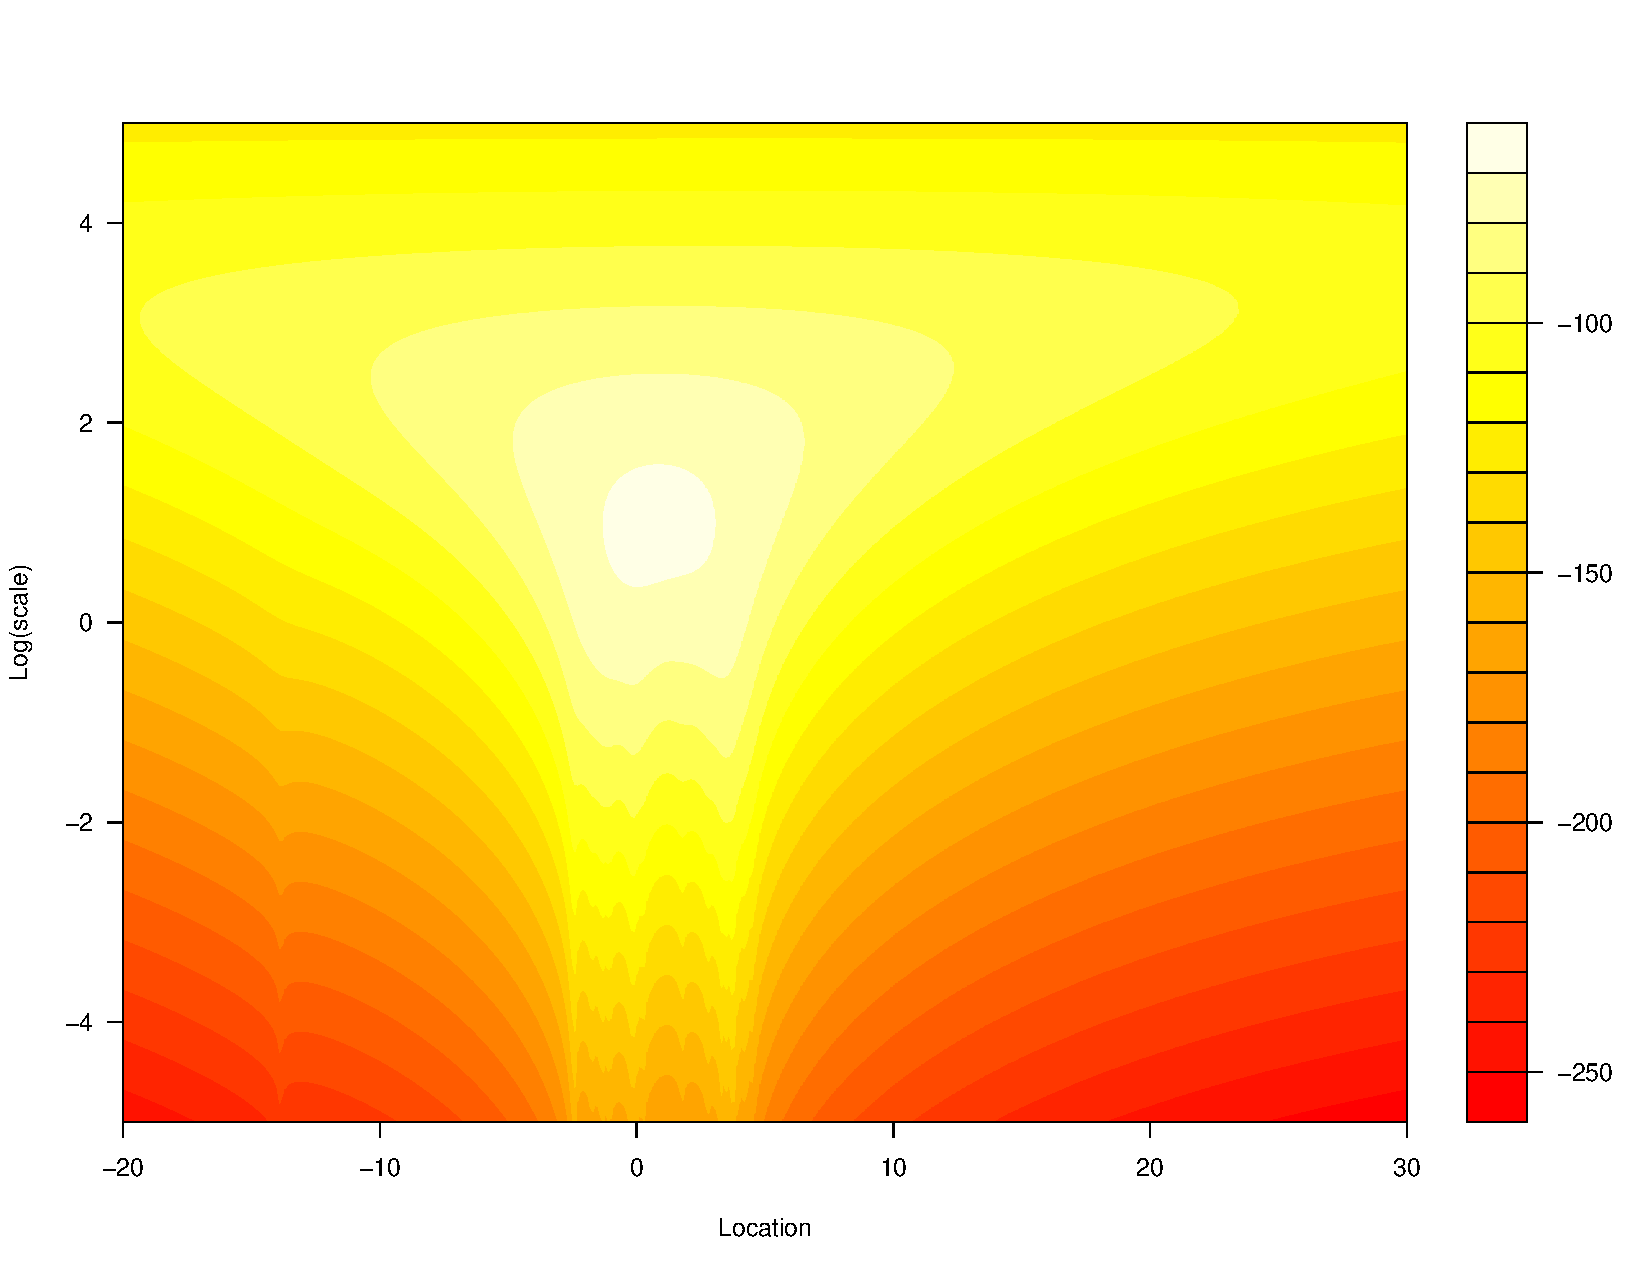
\includegraphics[scale=0.3]{figs/cauchy-loglik-2d.pdf}
\caption{Loglikelihood Function of $Cauchy(\theta, \sigma)$}
\label{img:cauchy-loglik-2d}
\end{figure}

\begin{figure}[h!]
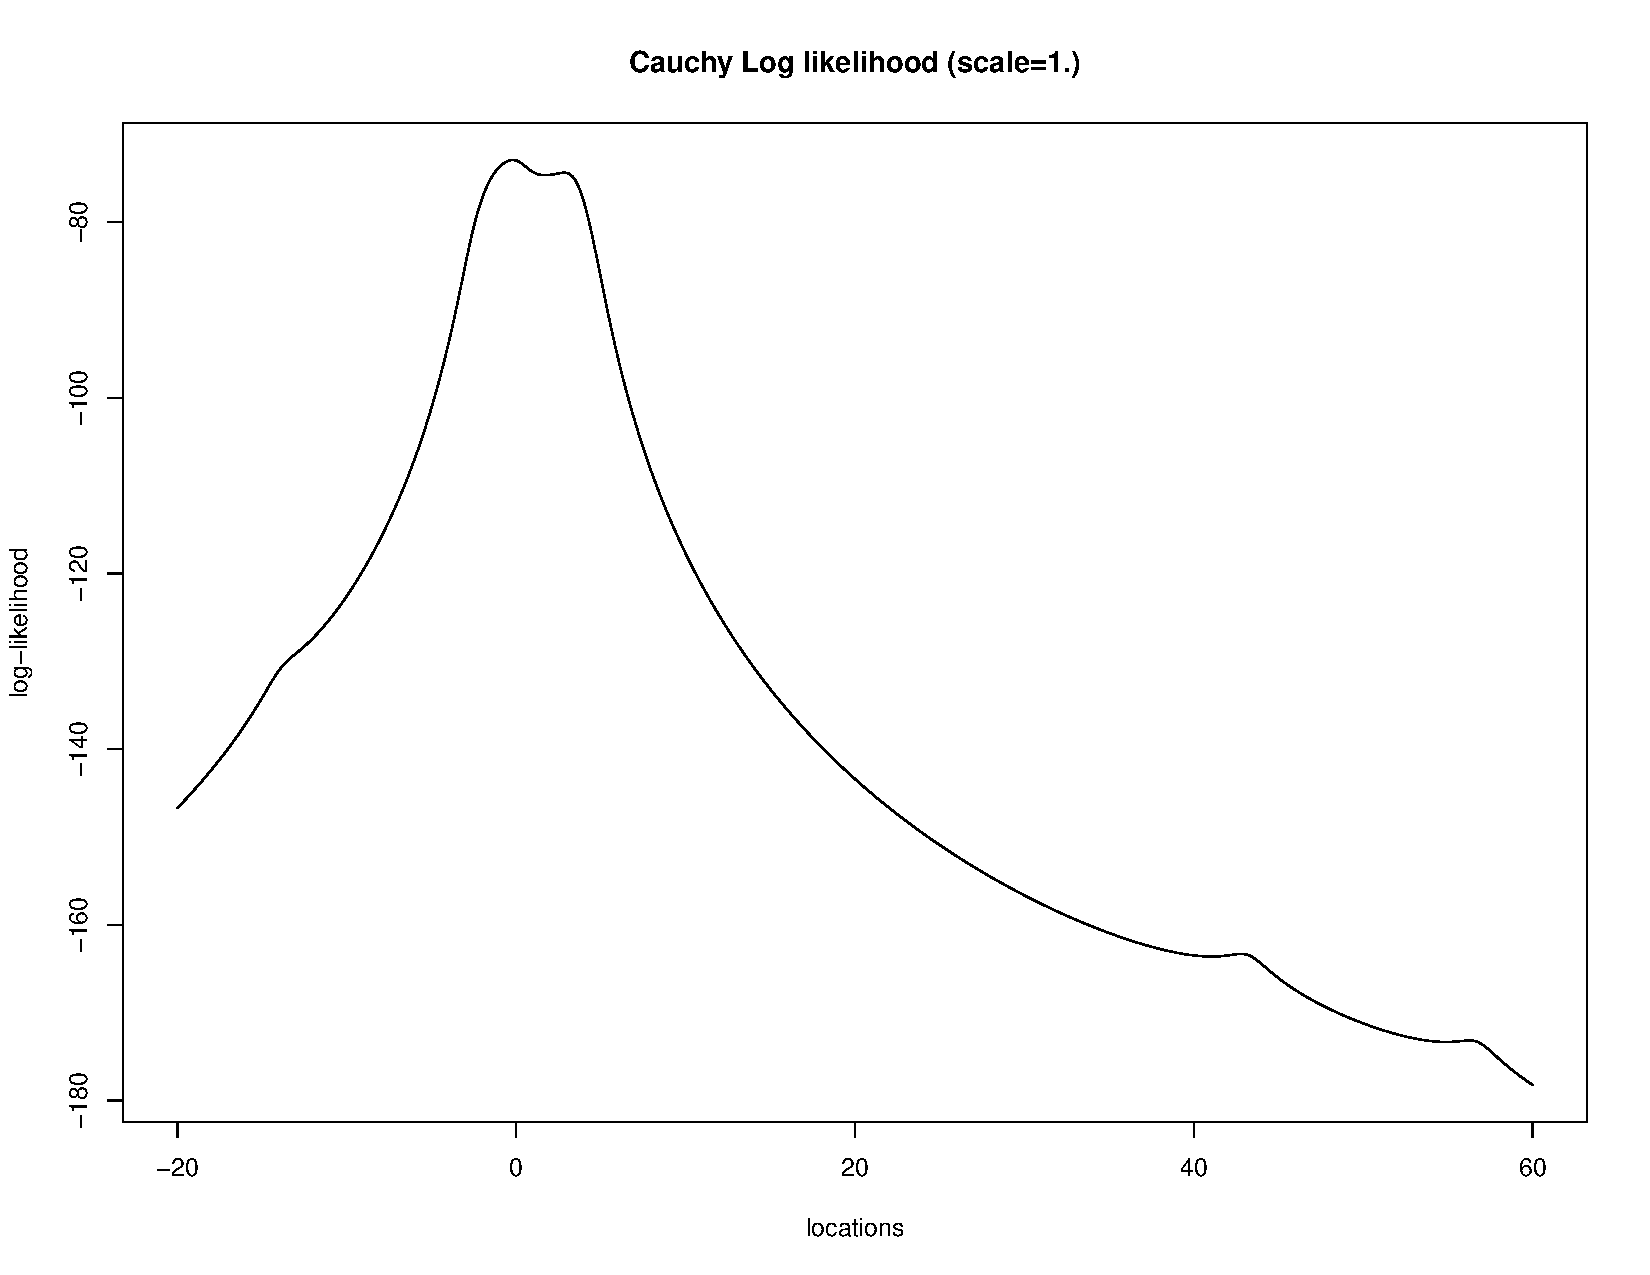
\includegraphics[scale=0.3]{figs/cauchy-loglik-1d.pdf}
\caption{Loglikelihood Function of $Cauchy(\theta, 1.)$}
\label{img:cauchy-loglik-1d}
\end{figure}

As we can easily it is an univariate optimization problem, we apply Maximum likelihood estimation (MLE) to maximize the real-valued log-likelihood function $g(x)$ of a Cauchy distribution $Cauchy(\theta, 1)$. Let's consider the location-scale family of Cauchy distribution whose PDFs are given by

$$f(x;\theta, \sigma) = \frac{1}{\pi \sigma} (1 + (\frac{x-\theta}{\sigma})^2)^{-1}$$

\begin{figure}[h!]
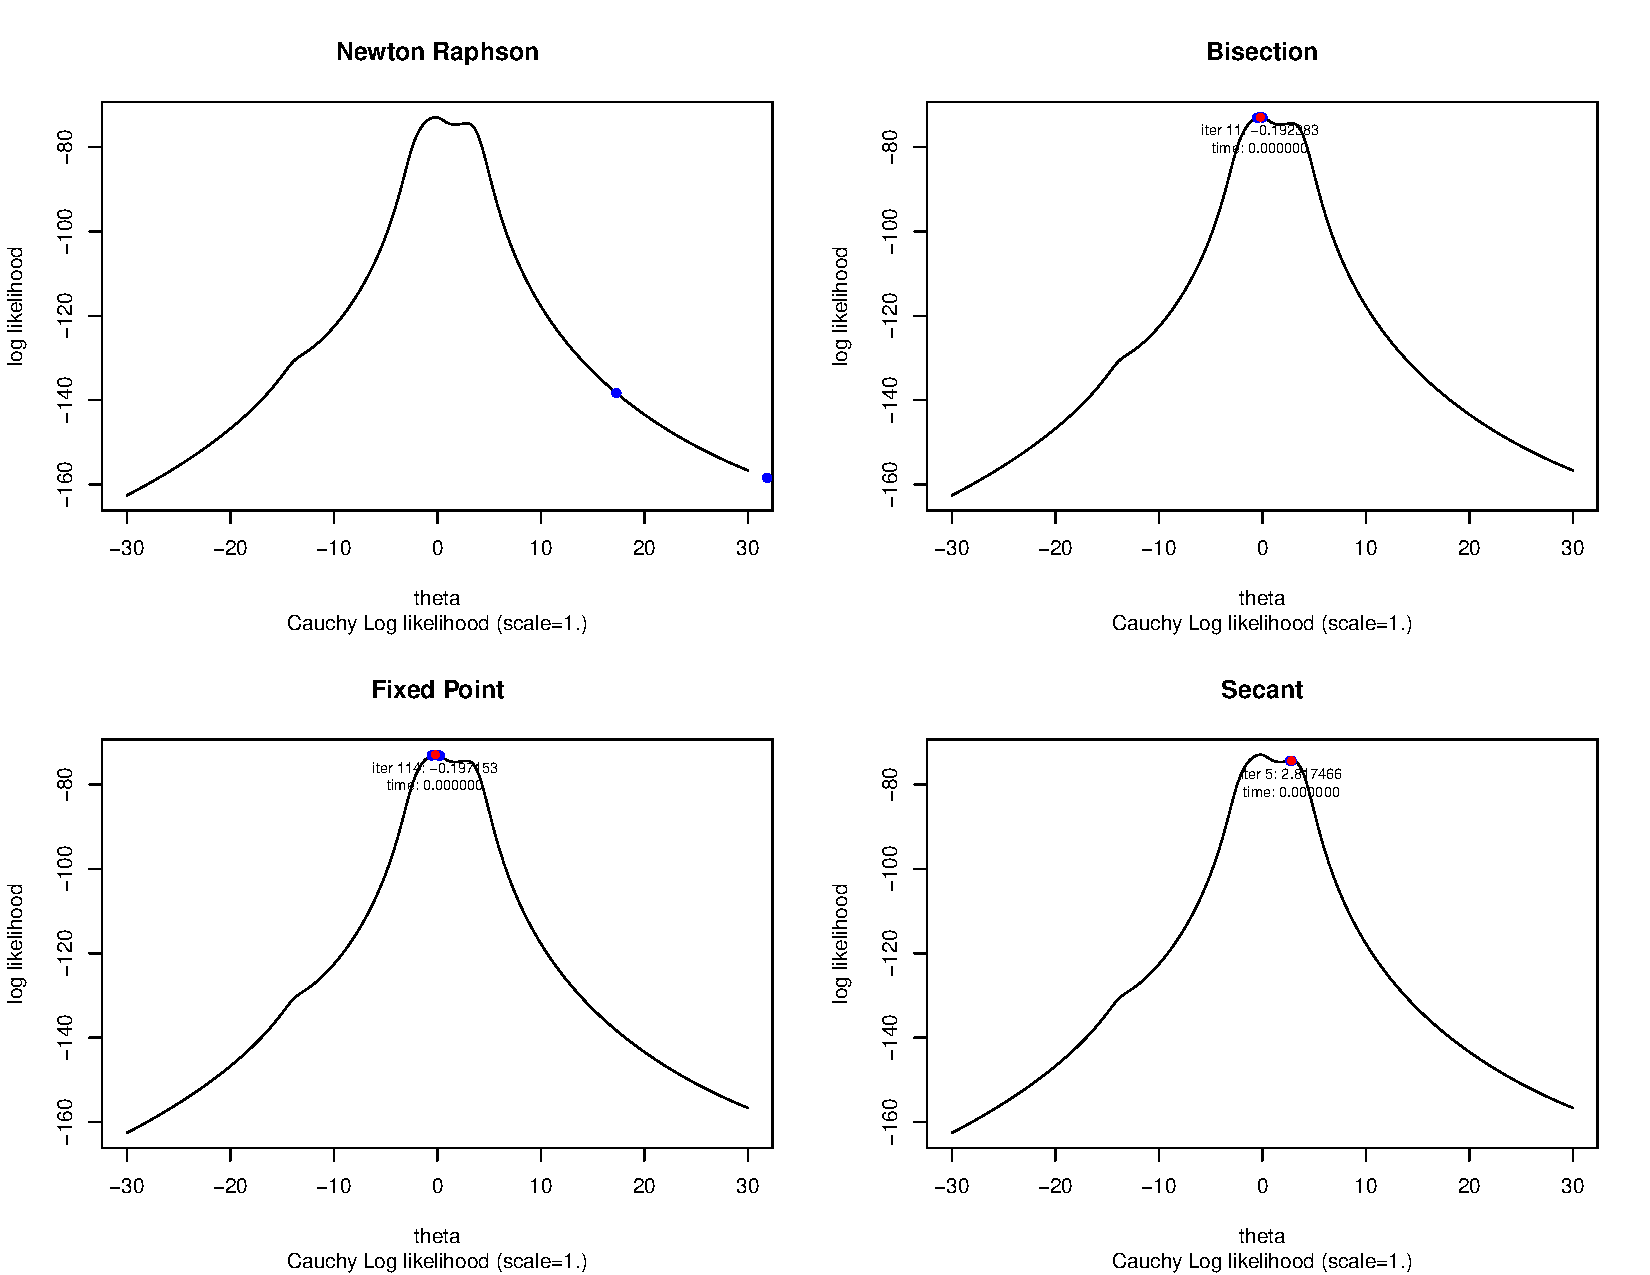
\includegraphics[scale=0.3]{figs/cauchy-sol-on-loglik-4figs.pdf}
\caption{The solutions and iterations traces of four MLE methods on the log-likelihood.}
\label{img:cauchy-sol-on-loglik-4figs}
\end{figure}

\begin{figure}[h!]
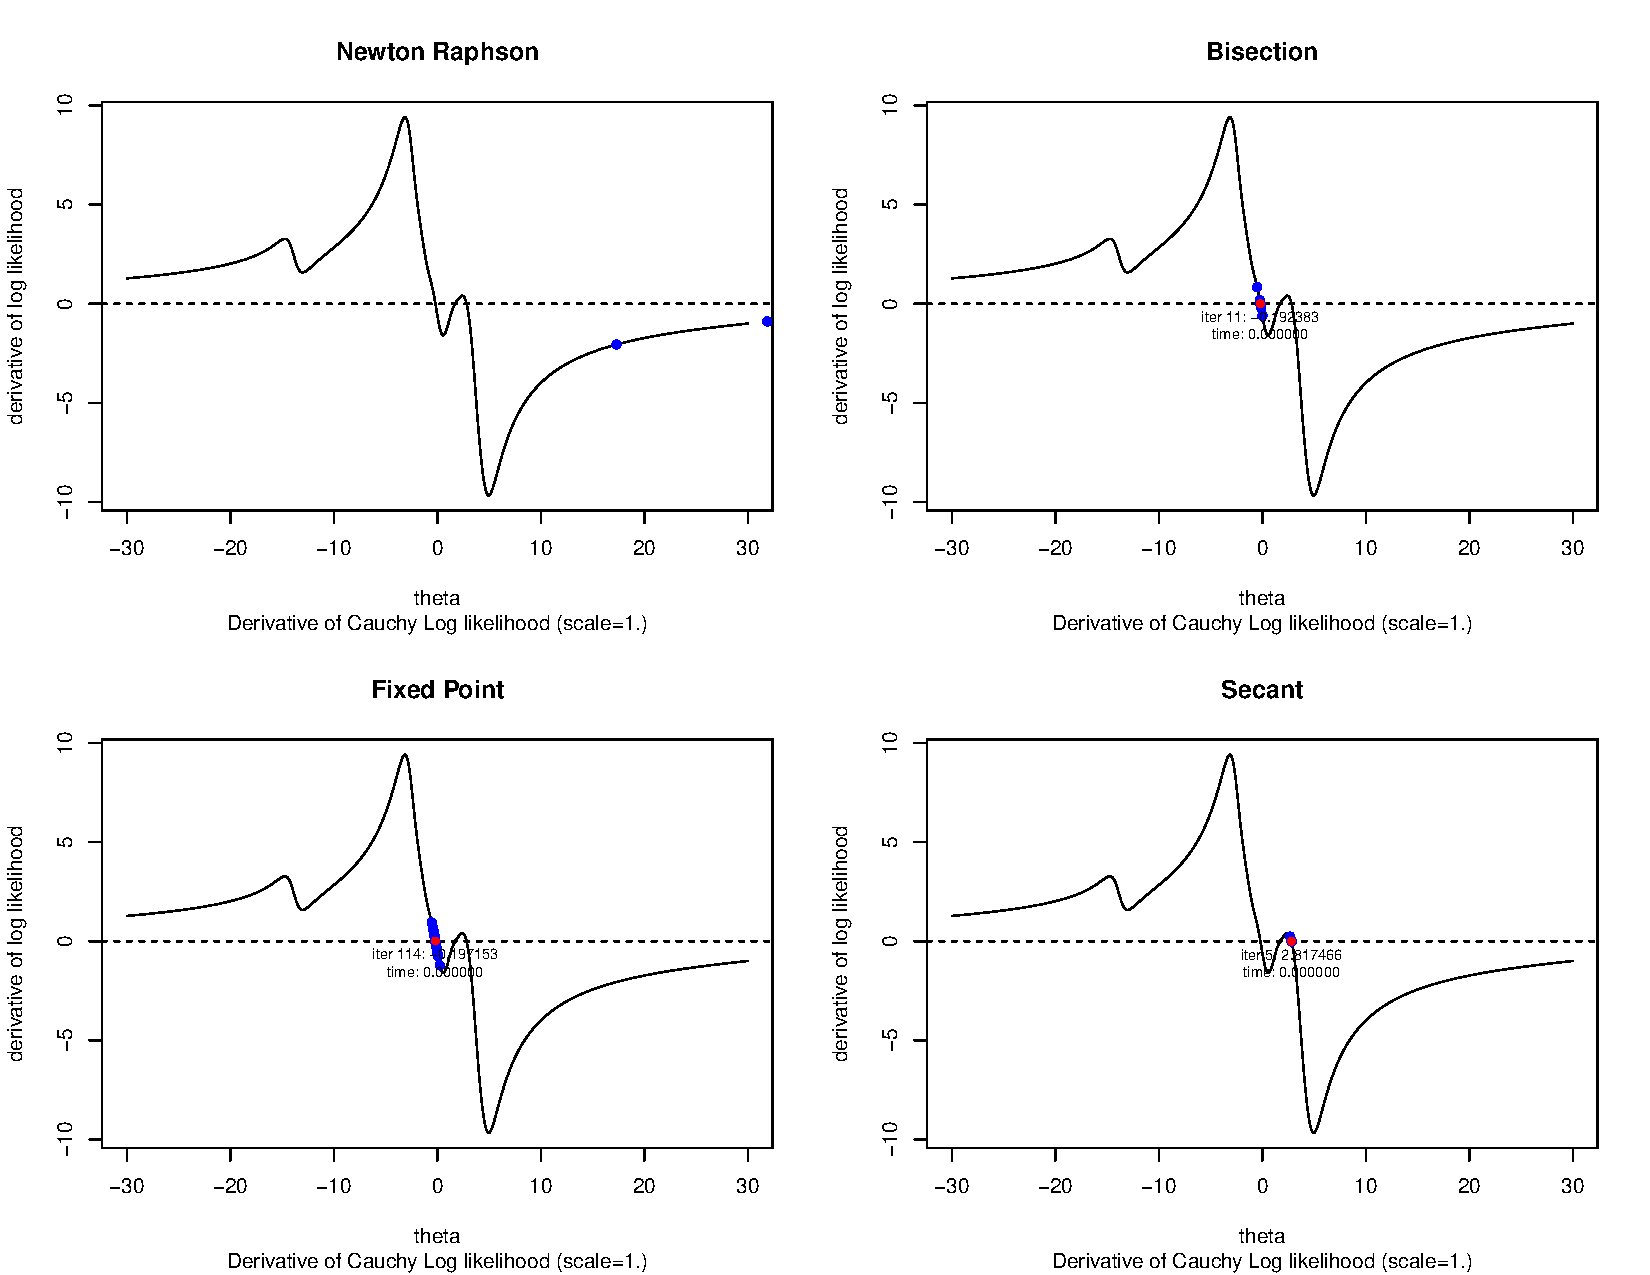
\includegraphics[scale=0.3]{figs/cauchy-sol-on-deriv-4figs.pdf}
\caption{The solutions and iterations traces of four MLE methods on the derivative of the log-likelihood.}
\label{img:cauchy-sol-on-deriv-4figs}
\end{figure}

where $\theta$ is its location and $\sigma$ is its scale, in our scenario, it equals to 1. By definition, the log-likelihood $\mathcal L$ of a batch of sample data (shown above), $x_i, i=1,2,3,\cdots,n$ is the logarithm of their probability, assuming the data are independently and idendically distributed according to $f(x; \theta, \sigma)$. The independence assumption implies the probability is the product of individous probabilities, whence

\vspace{-0.1in}
\begin{equation*}
\begin{split}
\mathcal L (\theta; \sigma=1, x) 
&= log \prod^{n}_{i=1} f(x_i; \theta, \sigma=1) \\
& = - \sum^{n}_{i=1} log(1+(\frac{x_i-\theta}{\sigma})^{2}) - n log(\pi\sigma).
\end{split}
\end{equation*}

\begin{figure}[h!]
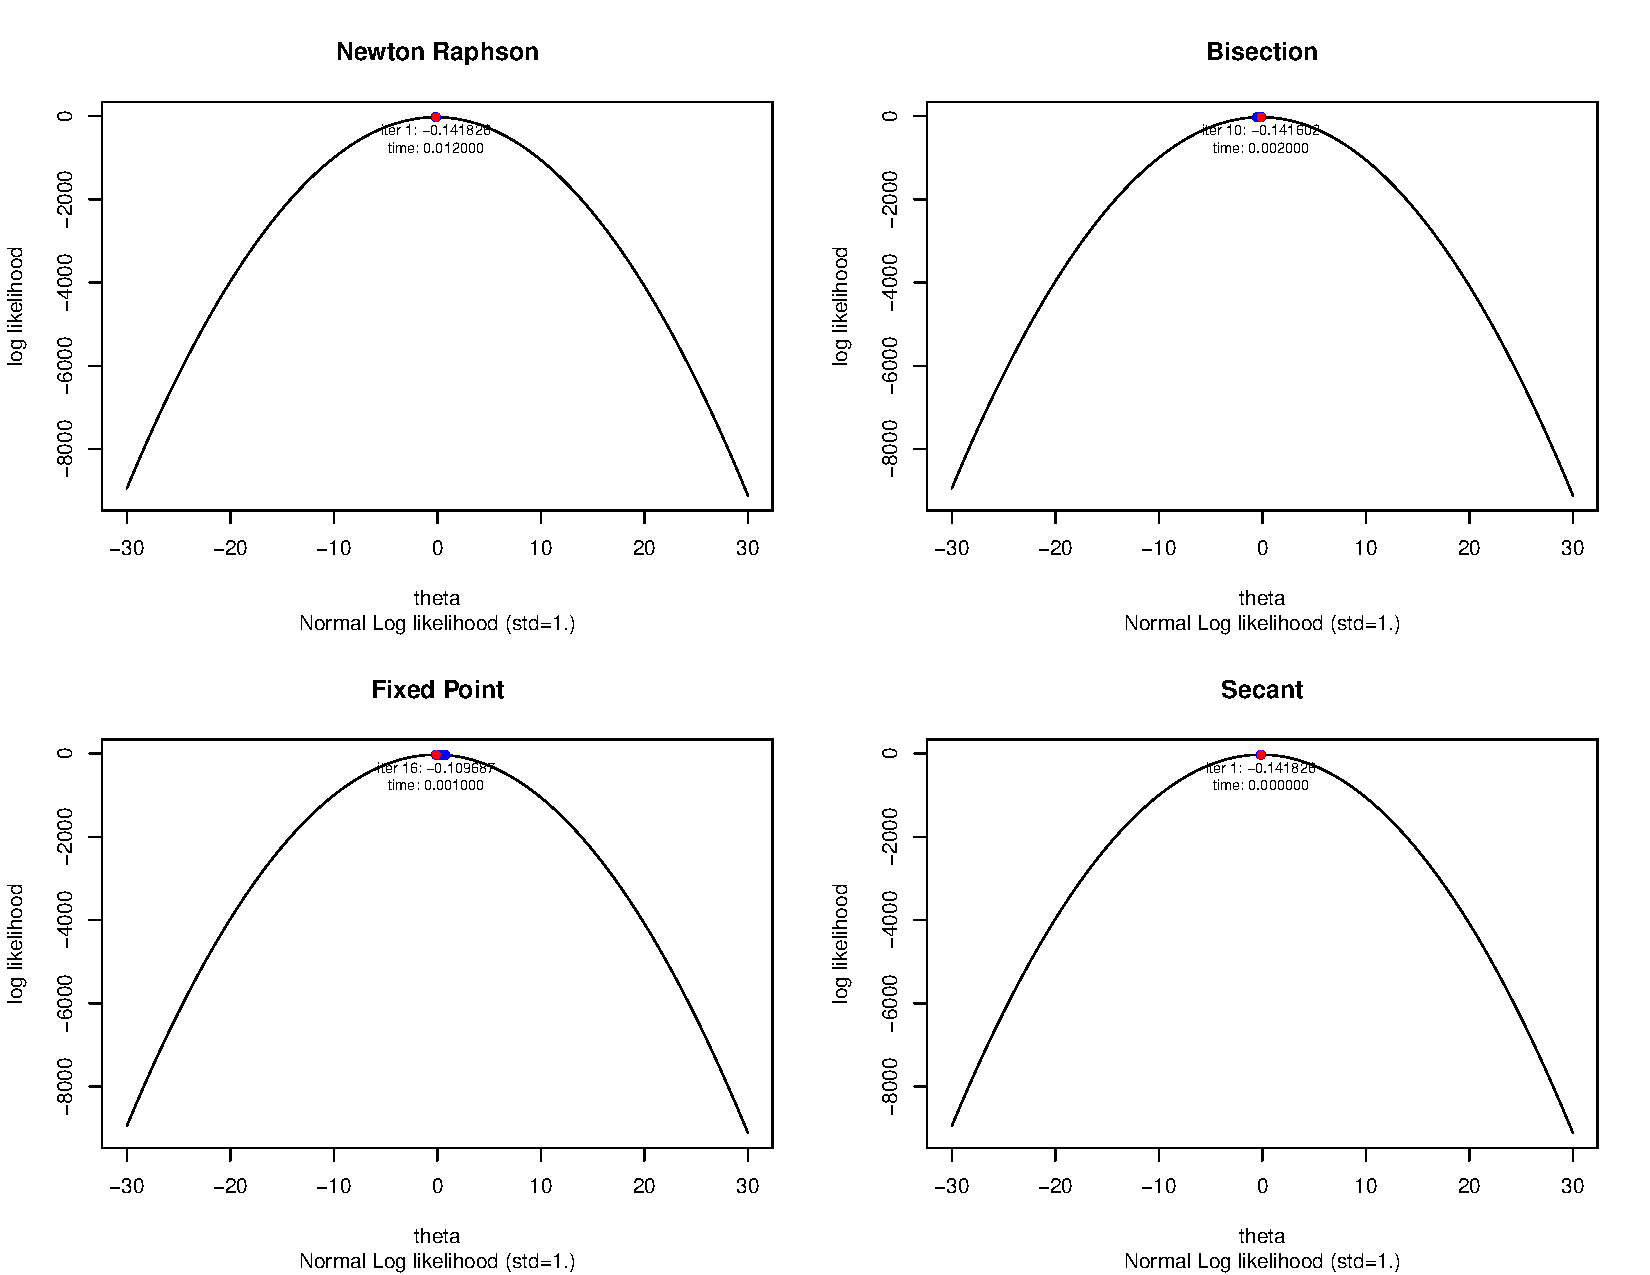
\includegraphics[scale=0.3]{figs/normal-sol-on-loglik-4figs.pdf}
\caption{The solutions and iterations traces of four MLE methods on the log-likelihood.}
\label{img:normal-sol-on-loglik-4figs}
\end{figure}

\begin{figure}[h!]
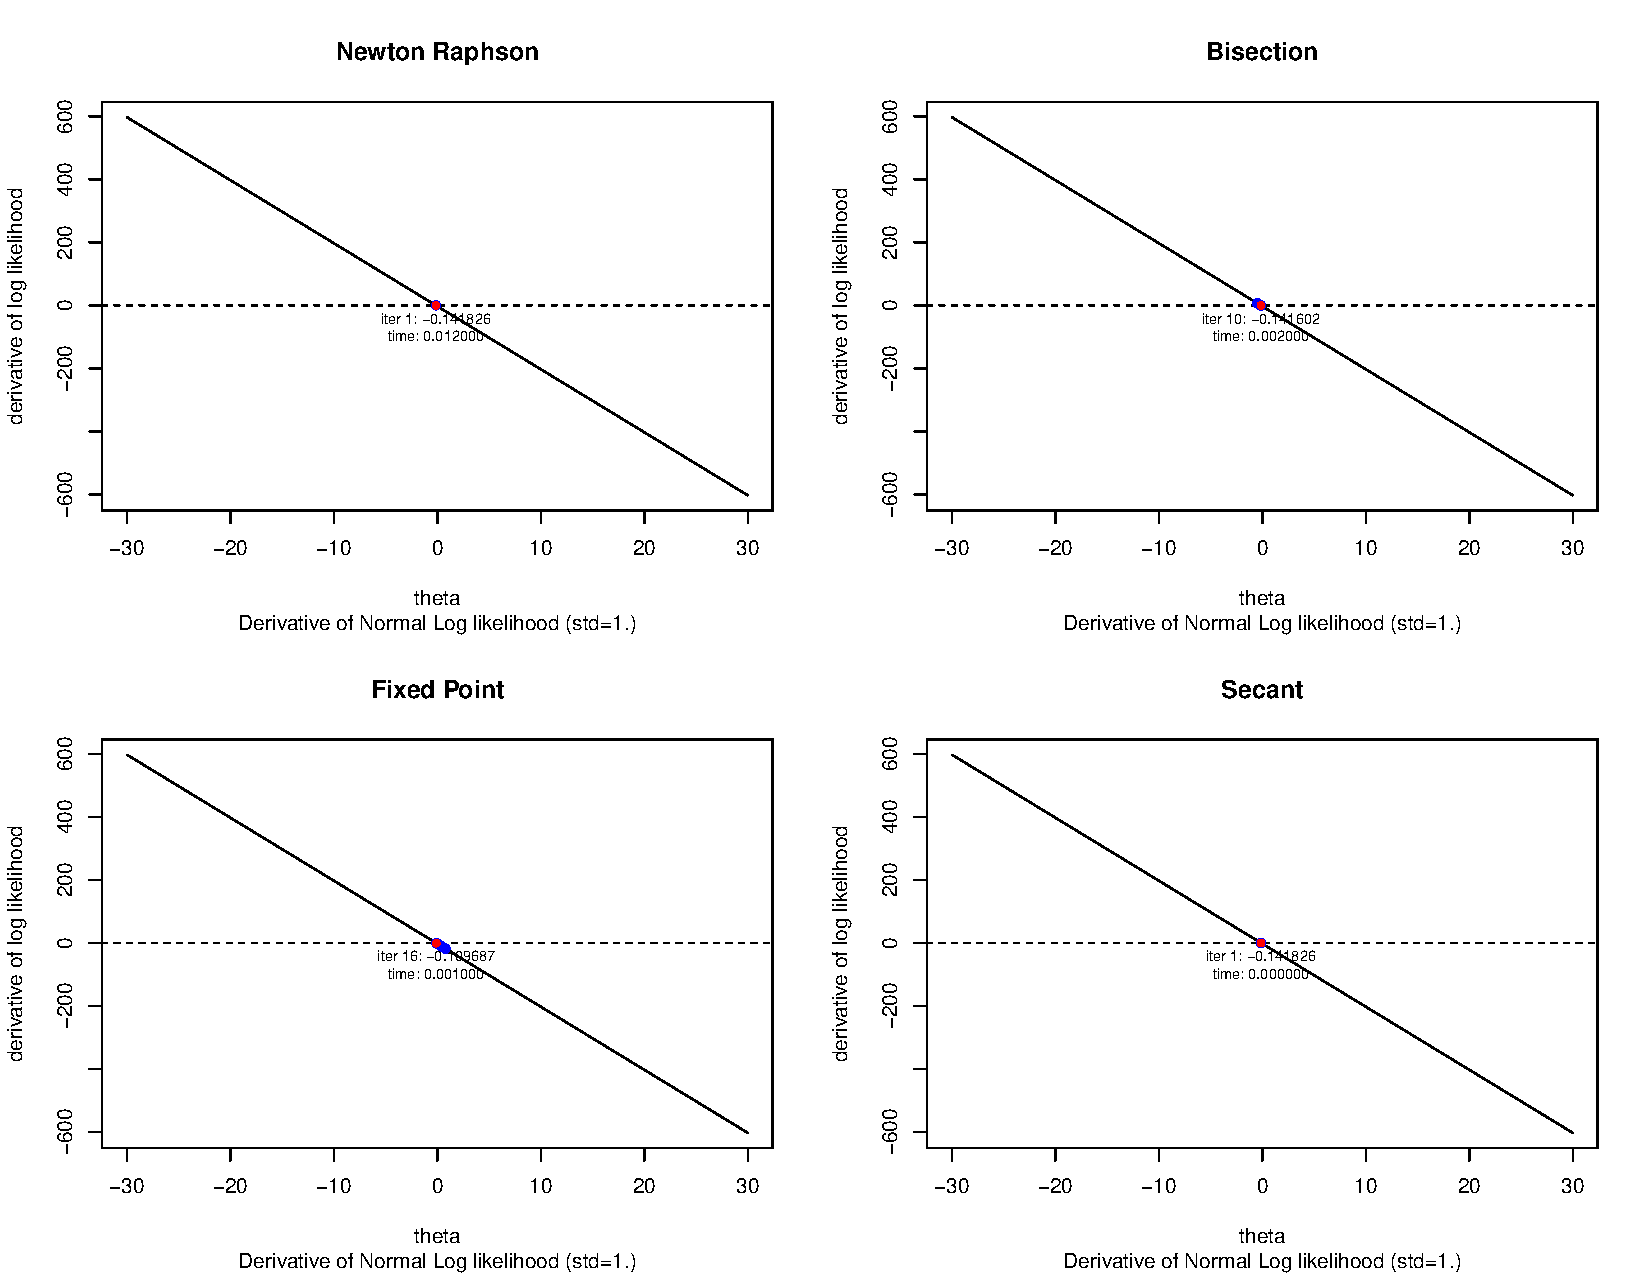
\includegraphics[scale=0.3]{figs/normal-sol-on-deriv-4figs.pdf}
\caption{The solutions and iterations traces of four MLE methods on the derivative of the log-likelihood.}
\label{img:normal-sol-on-deriv-4figs}
\end{figure}

In order to understand the physics behind univariate optimization better, we manually implement four methods for \textit{Raphson Newton Method}, \textit{Bisection Method}, \textit{Fixed Point Iteration} and \textit{Secant Method} respectively in \textit{findroot.R} of Appendix \ref{appendix:findroot}. In our \textbf{R} code, We use \code{numDeriv} package to solve the first derivative for our self-defined log-likelihood functions. For Problem 2.1 from \textit{(a)} to \textit{(d)}, we plot our solutions for these fours methods on the log-likelihood function of Cauchy distribution (shown in Fig. \ref{img:cauchy-sol-on-loglik-4figs}) and its derivatives (shown in Fig. \ref{img:cauchy-sol-on-deriv-4figs}) respectively.


In problem 2.1 \textit{(e)}, we also apply same methods to a random sample of size 20 from a $N(\theta, 1)$ distribution by using function \code{rnorm} in \textbf{R}. We likewise model these randomly generated data points with MLE . The PDF of a Normal distribution is

$$f(x; \mu, \sigma) = (2 \pi \sigma^2) ^ (-1/2) exp(-\frac{1}{2} \frac{(x-\mu)^2}{\sigma^2})$$

where $\mu$ is mean and $\sigma^2$ is variance, which are the two parameters that need to be estimated. Therefore, the log-likelihood function can be expressed as

$$\mathcal L (\mu; \sigma=1, x) = - \frac{n}{2} ln(2 \pi) - \frac{n}{2} ln(\sigma^2) - \frac{1}{2 \sigma^2} \sum_{i=1}^{n} (x_i-\mu)^2$$


In Fig. \ref{img:cauchy-sol-on-loglik-4figs}, Fig. \ref{img:cauchy-sol-on-deriv-4figs}, Fig\ref{img:normal-sol-on-loglik-4figs} and Fig. \ref{img:normal-sol-on-deriv-4figs}the red points mean the final solution for corresponding methods, and following a trace of blue points mean the history of iteration when finding the roots. According to the experiments, the local optimal point is highly depended on its initial choices. We can draw some same conclusions from these experiments. For example, \textit{Fisher Scoring Iterations} generally makes rapid improvements initially, while Newton-like method gives better refinements near the end, however, sometime accoring to our observations, Newton-like method cannot get valid solution when the starting point is too far away from the true optimal point. Regarding \textit{Fixed Points Iteration} usually takes more steps to get convergence. Instead, \textit{Bisection} and \textit{Secant} Method can get convergence within very few steps. In terms of the speed of computation, it is really hard to differentiate these four method when dealing with the log-likelihood of Cauchy, but \textit{Secant} has an clear edge over the other three methods. 

\section{Problem 2.5}

In problem 2.5, there were 46 crude oil spills of at least 1,000 barrels from tankers in U.S. waters during 1974-1999. The website for this book contains the following data: the number of spills in the $i$-th year, $N_i$; the estimated amount of oil shipped through US waters as part of US import/export operations in the $i$-th year, adjusted for spillage in international or foreign waters, $b_{i1}$; and the amount of oil shipped through U.S. waters during domestic shipments in the $i$-th year, $b_{i2}$. The data are adapted from. Oil shipment amounts are measured in billions of barrels (Bbbl). The volume of oil shipped is measure of exposure to spill risk. Suppose we use the Possion process assumption given by $N_i | b_{i1}, b_{i2} \sim Possion(\lambda_i)$ where $\lambda_i = \alpha_1 * b_{i1} + \alpha_2 * b_{i2}$. The parameters of this model are $\alpha_1$ and $\alpha_2$, which represent the rate of spill occurence per Bbbl oil shipped during import/expert and domestic shipments, respectively. 

\begin{figure}[h!]
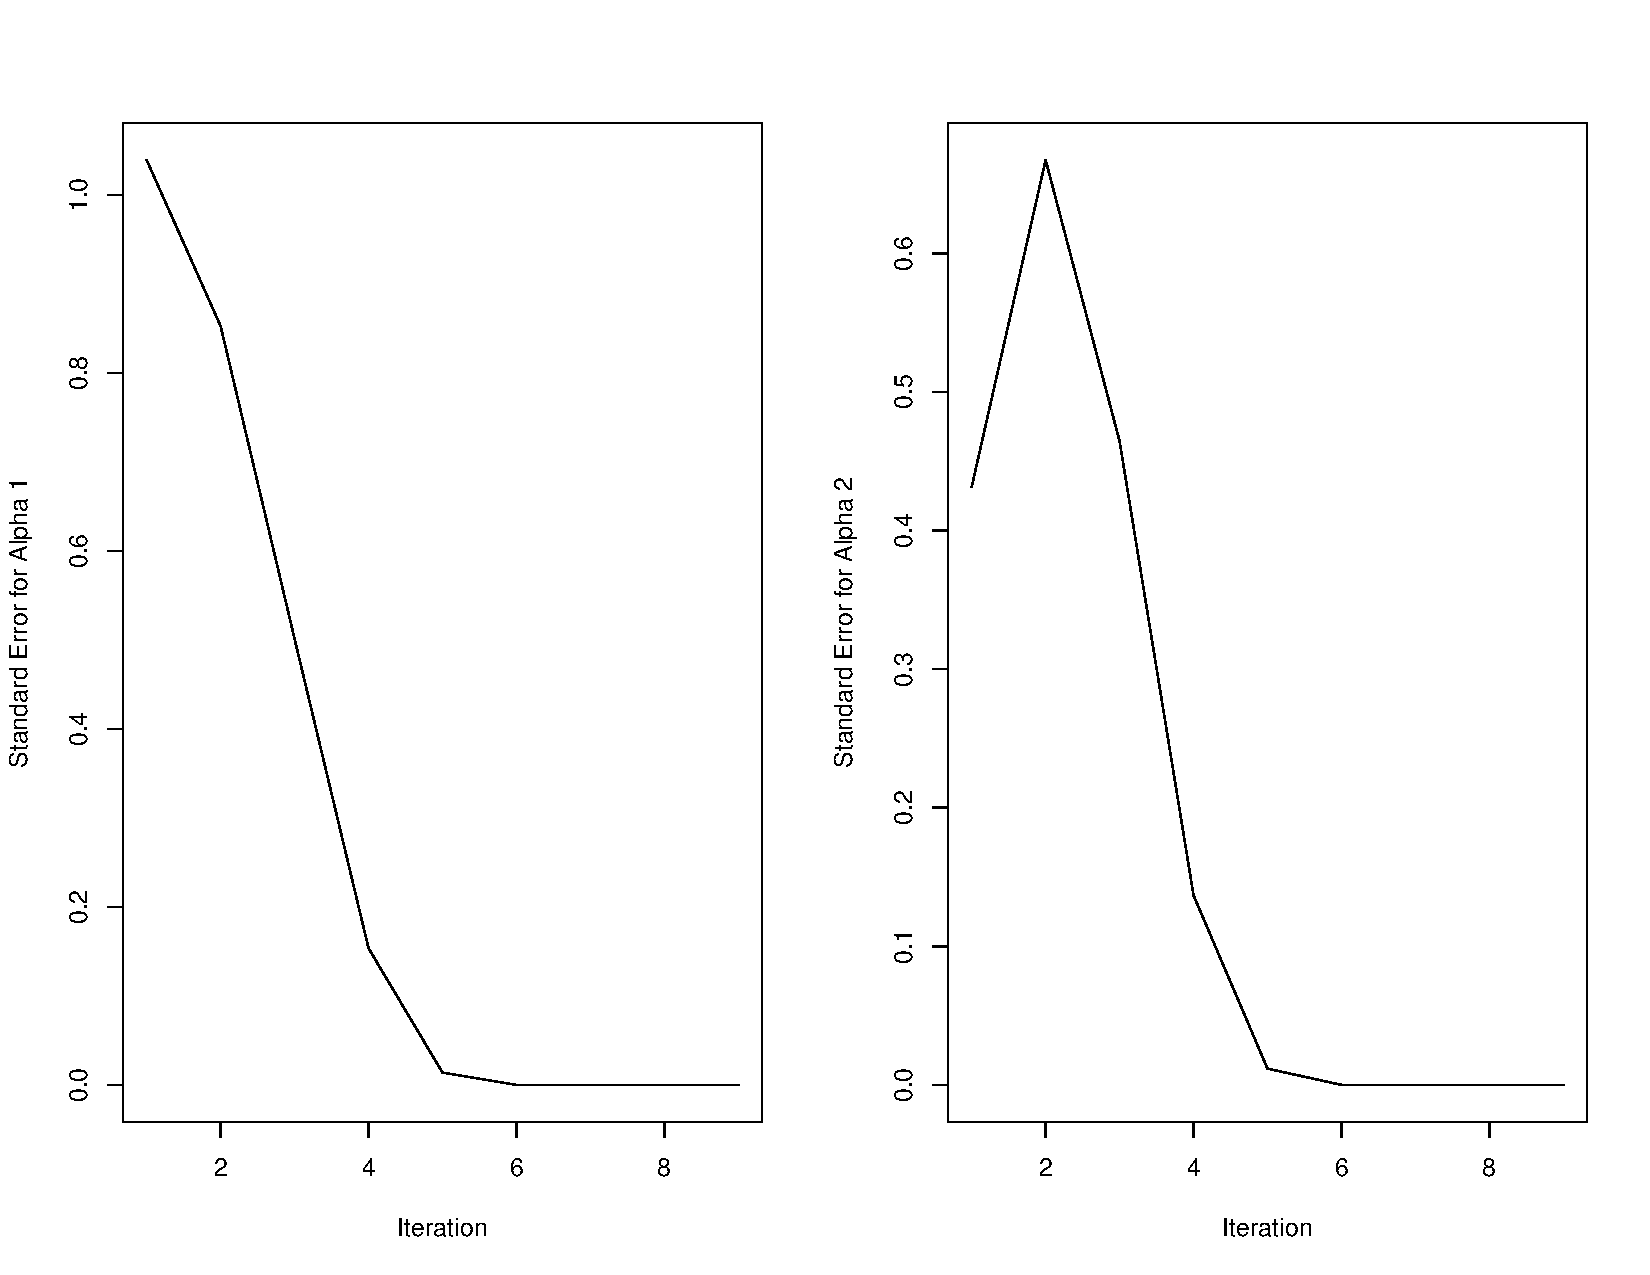
\includegraphics[scale=0.3]{figs/std-err-alpha.pdf}
\caption{Standard error of $\alpha$ over iterations.}
\label{img:std-err-alpha}
\end{figure}

\begin{figure}[h!]
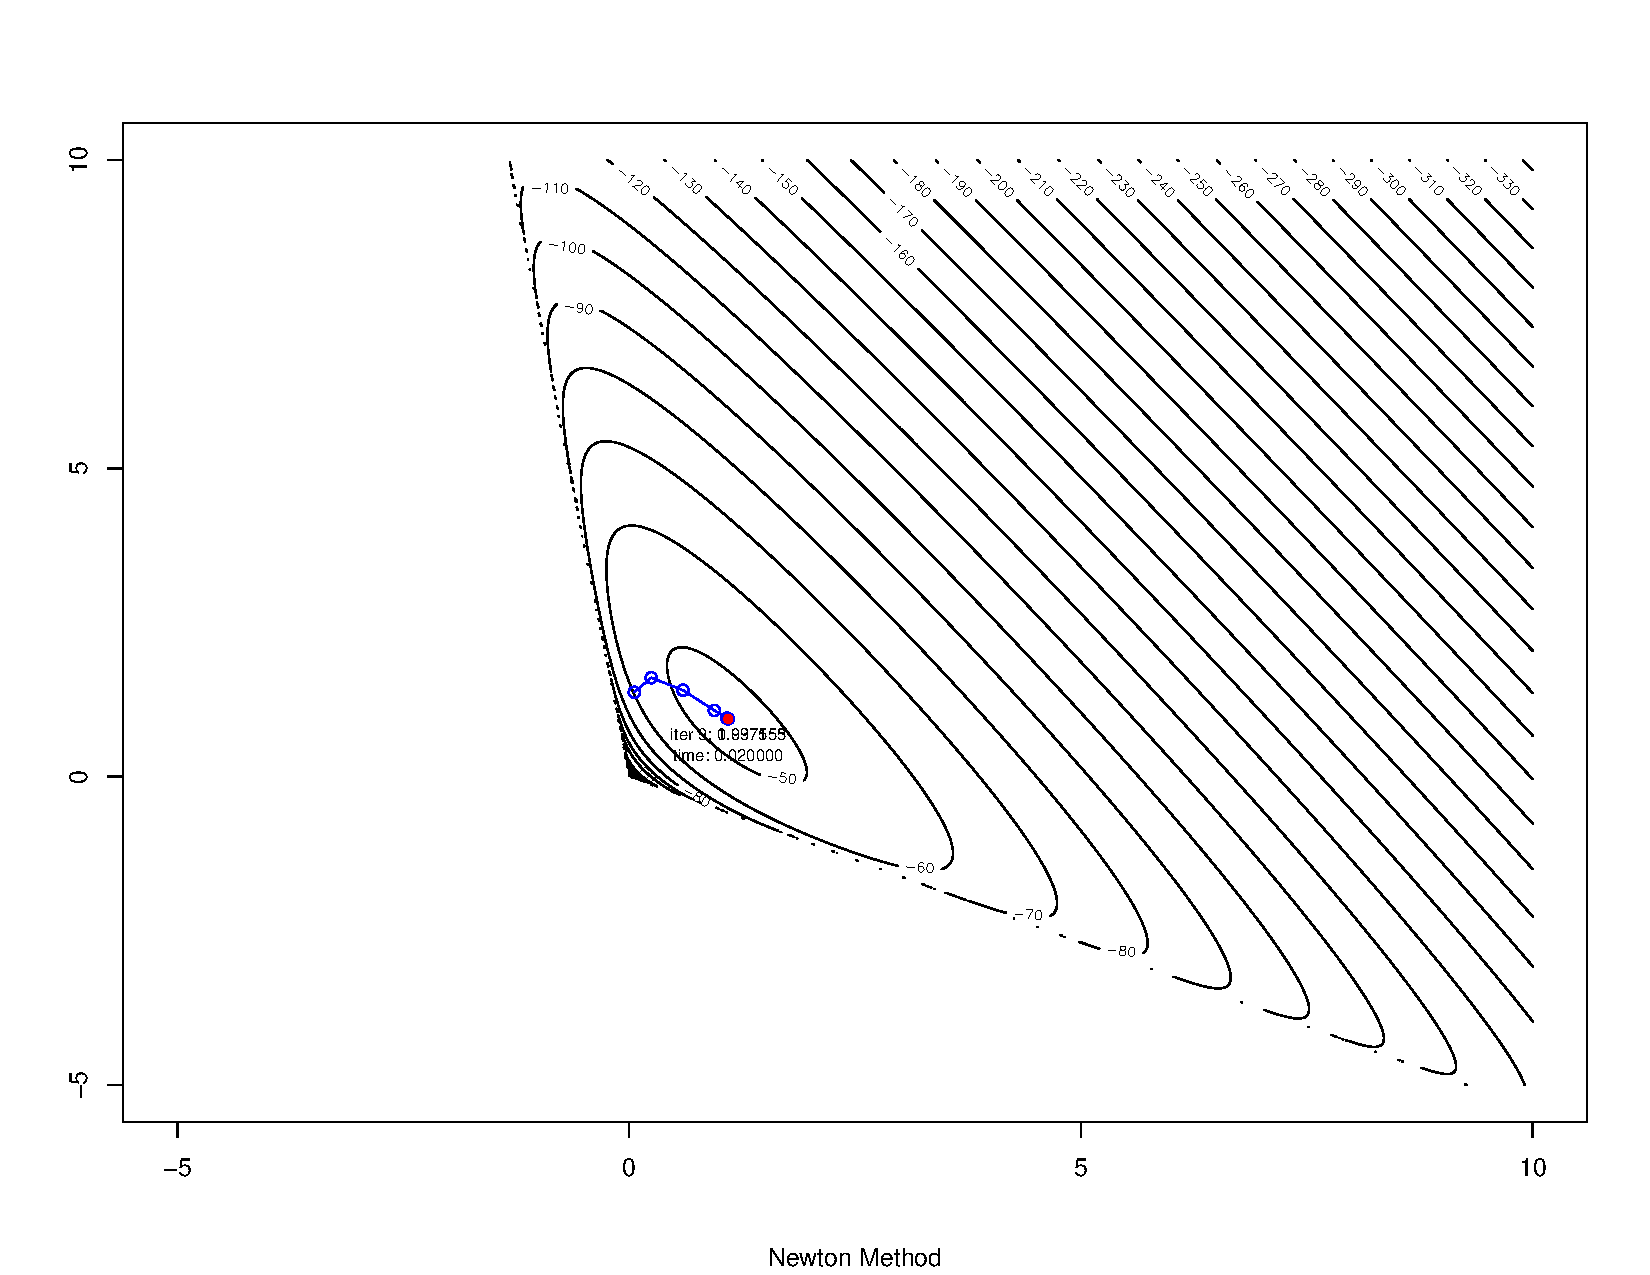
\includegraphics[scale=0.3]{figs/newton.pdf}
\caption{Newton Method.}
\label{img:newton}
\end{figure}

\begin{figure}[h!]
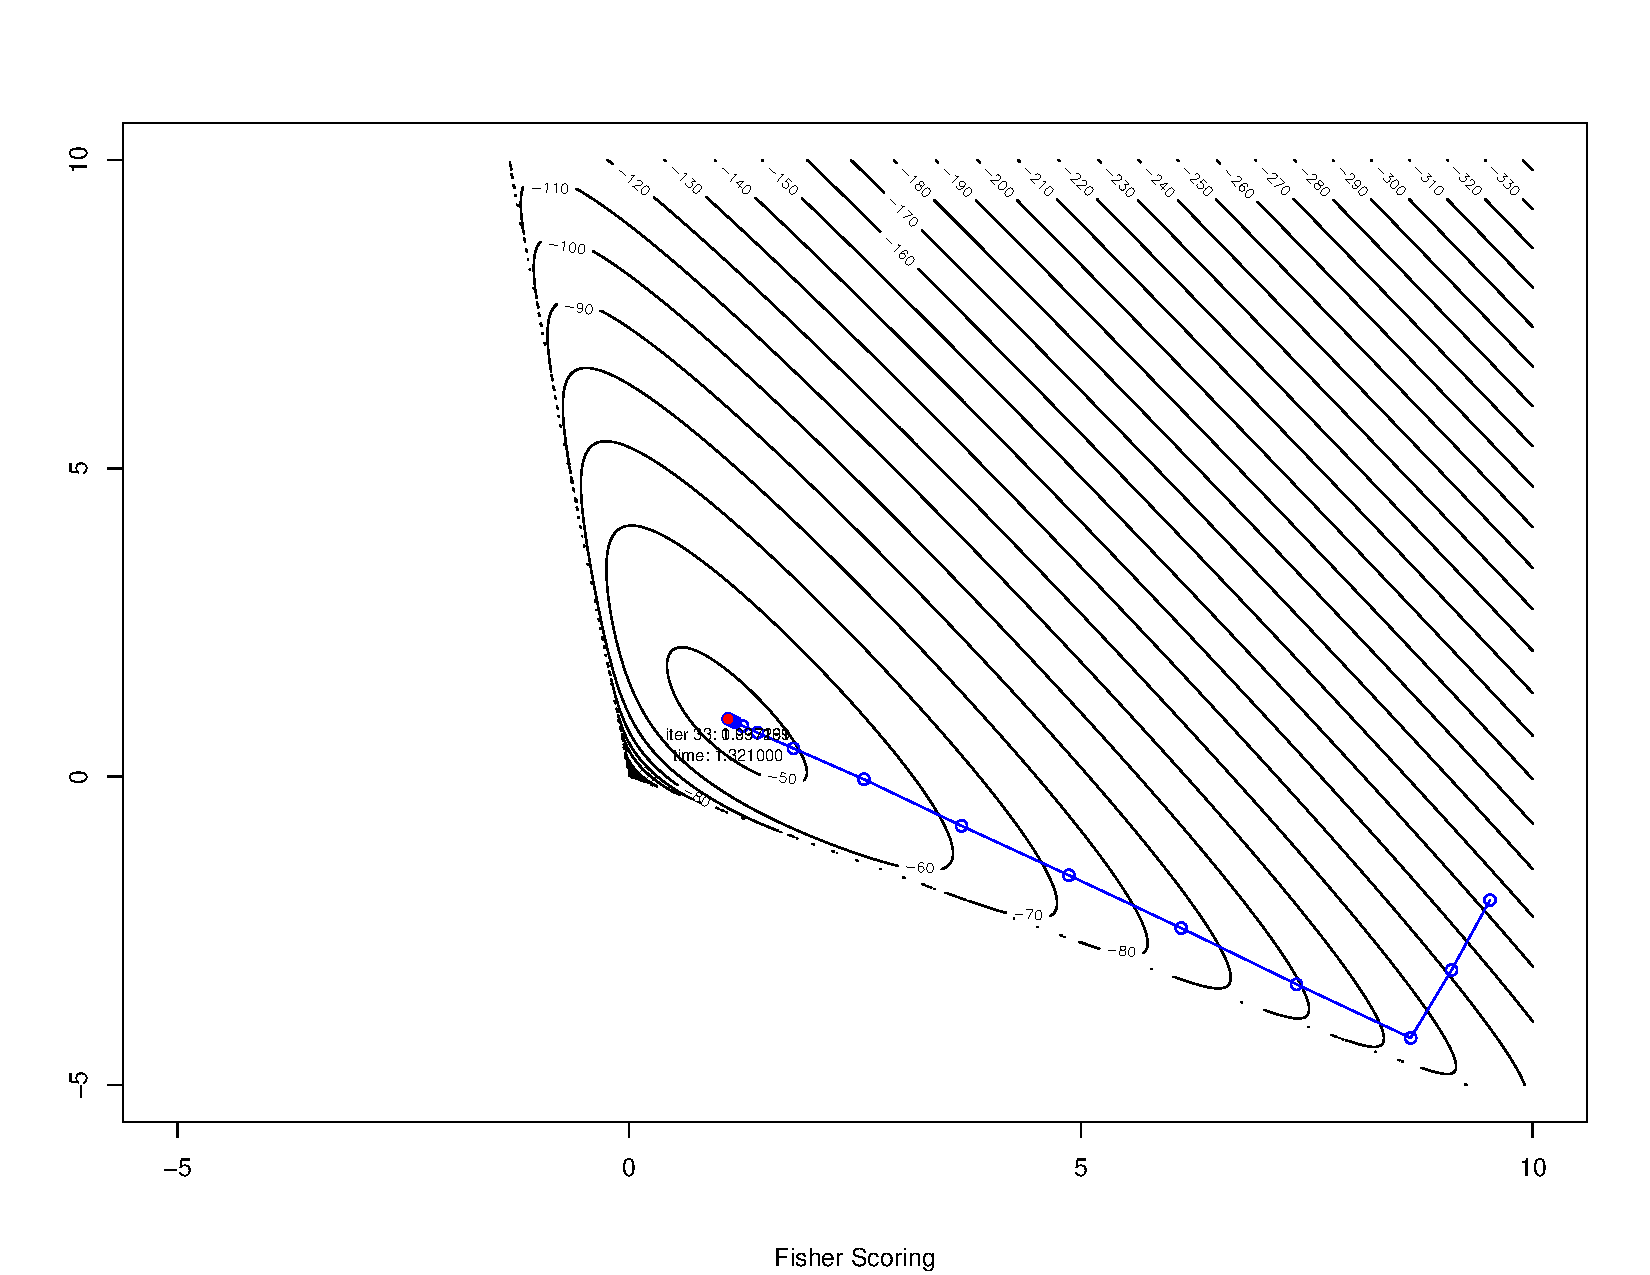
\includegraphics[scale=0.3]{figs/fisher.pdf}
\caption{Fisher Scoring.}
\label{img:fisher}
\end{figure}

Thus, according to definition, the probability mass function of a term of the sequence $x$ is 

$$p_i(N_i)=
\begin{cases}
\frac{(\alpha_1 b_{i1} + \alpha_2 b_{i2})^x e^{-\alpha_1 b_{i1} + \alpha_2 b_{i2}}}{N_i!},  & \text{if} N_i \in \Bbb Z_{+}\\
0,  & \text{if} x \notin \Bbb Z_{+}
\end{cases}
$$

And the log-likelihood function is

\vspace{-0.1in}
\begin{equation*}
\begin{split}
\mathcal L (\alpha_1, \alpha_2; N_i, b_{i1}, b_{i2})
&= - n (\alpha_1 b_{i1} + \alpha_2 b_{i2}) \\
& - \sum_{i=1}^{n} ln(N_i!) + ln(\alpha_1 b_{i1} + \alpha_2 b_{i2}) \sum_{i=1}^{n} x_i.
\end{split}
\end{equation*}

\begin{figure}[h!]
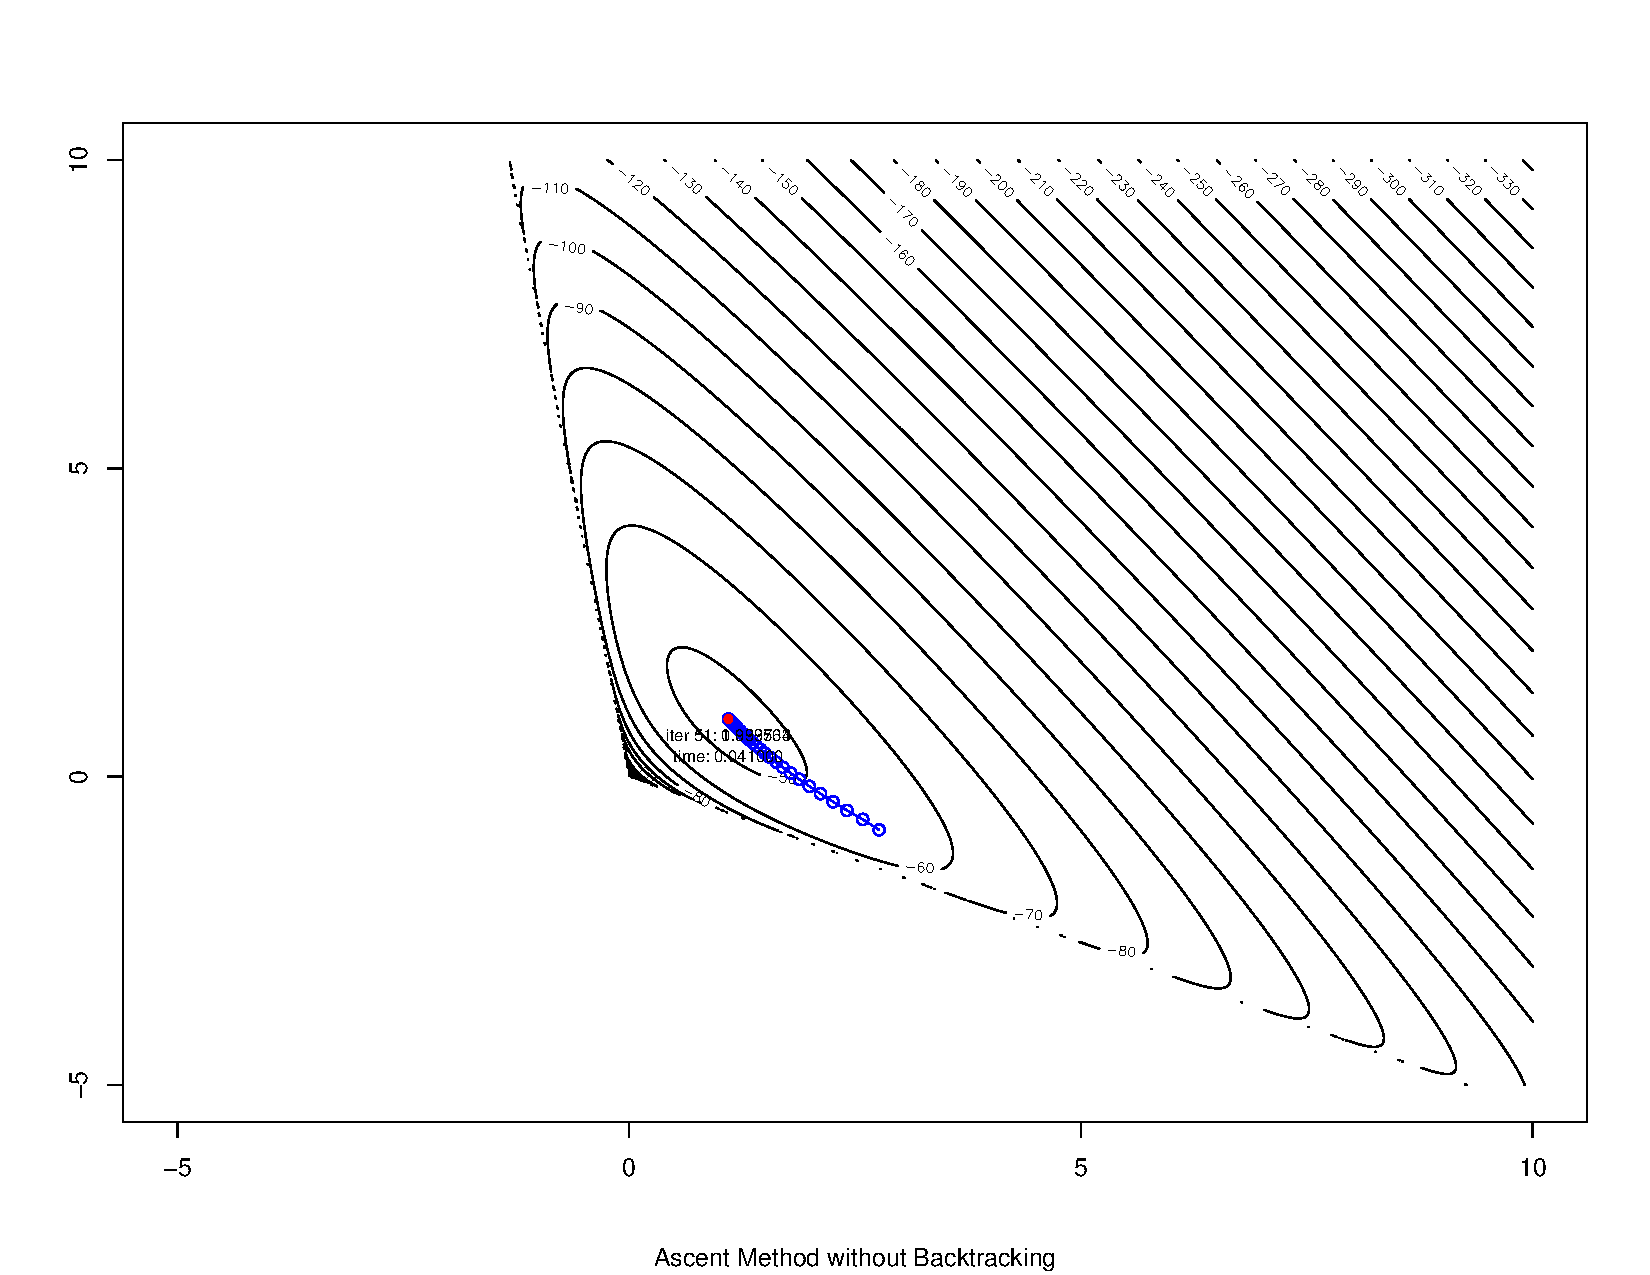
\includegraphics[scale=0.3]{figs/ascent-noback.pdf}
\caption{Steepest ascent method without backtracking.}
\label{img:ascent-noback}
\end{figure}

\begin{figure}[h!]
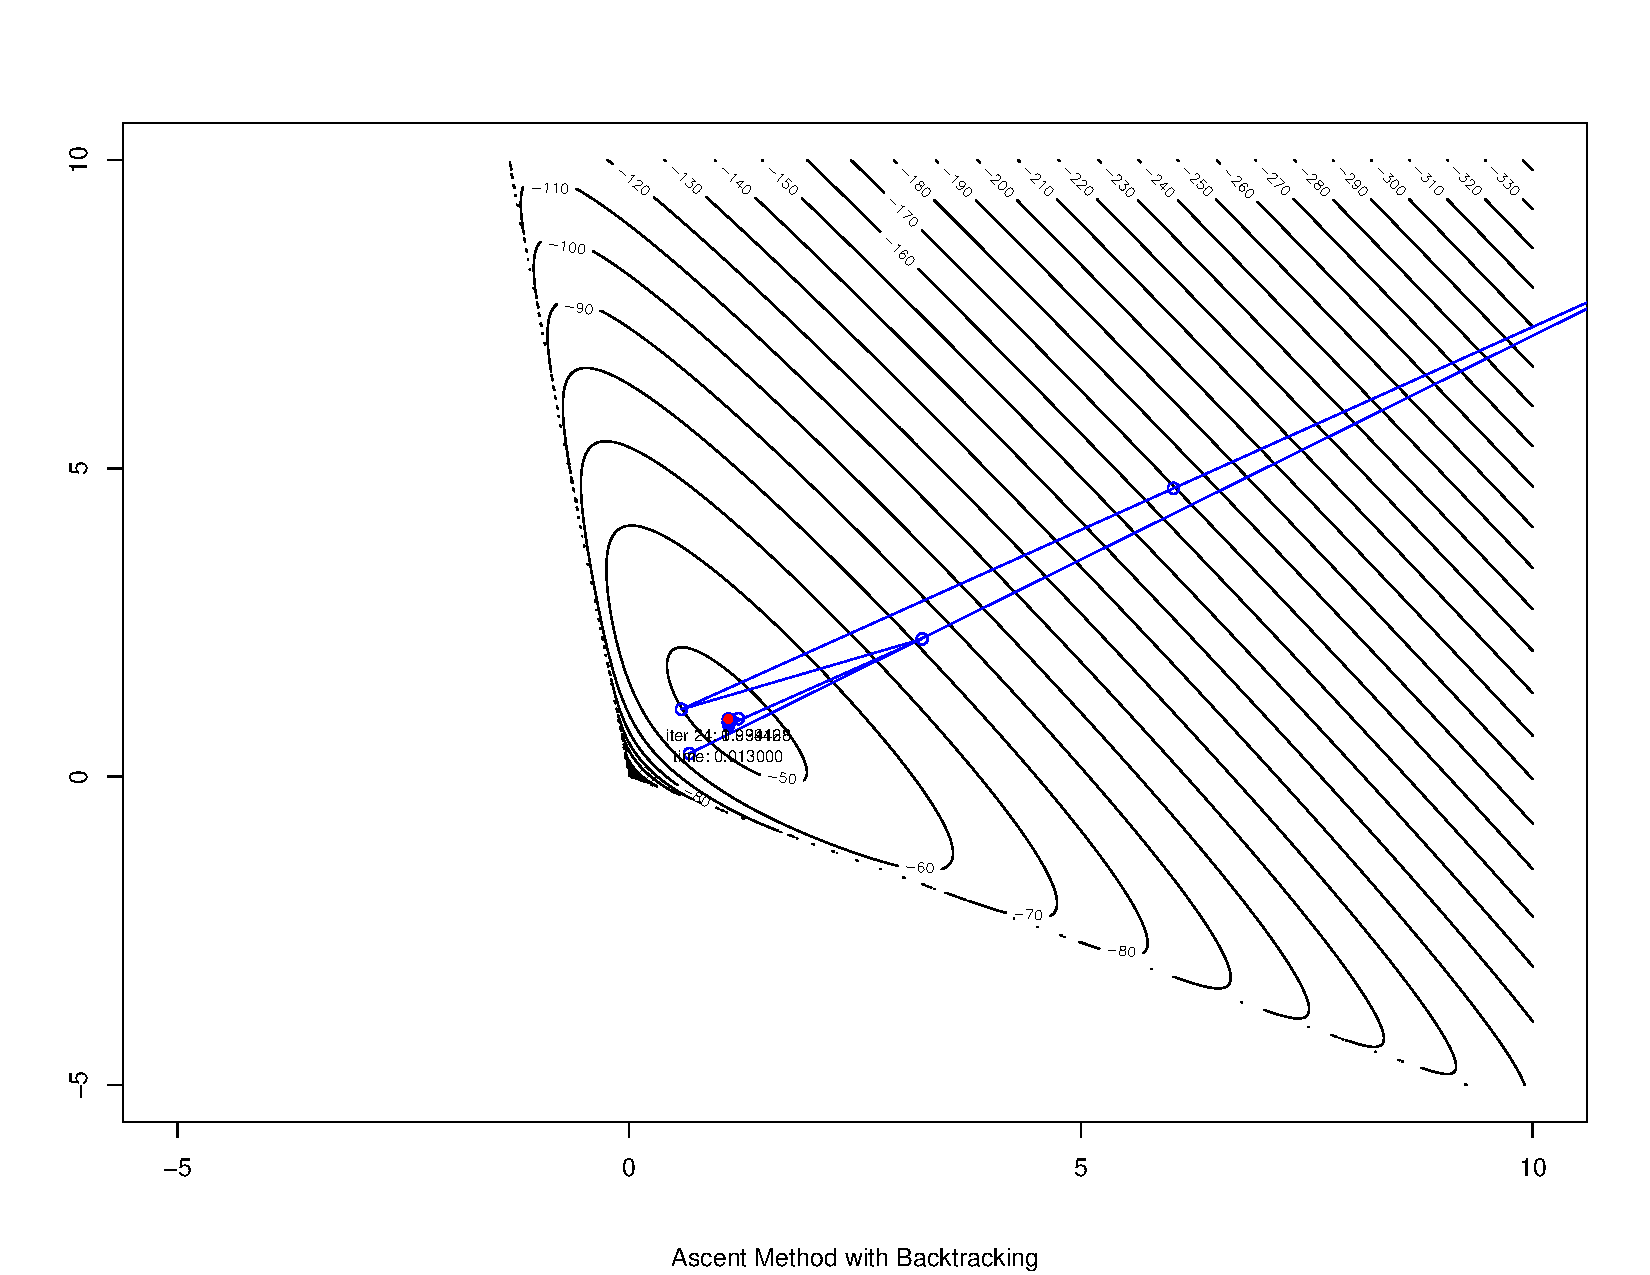
\includegraphics[scale=0.3]{figs/ascent-back.pdf}
\caption{Steepest ascent method with backtracking.}
\label{img:ascent-back}
\end{figure}

\begin{figure}[h!]
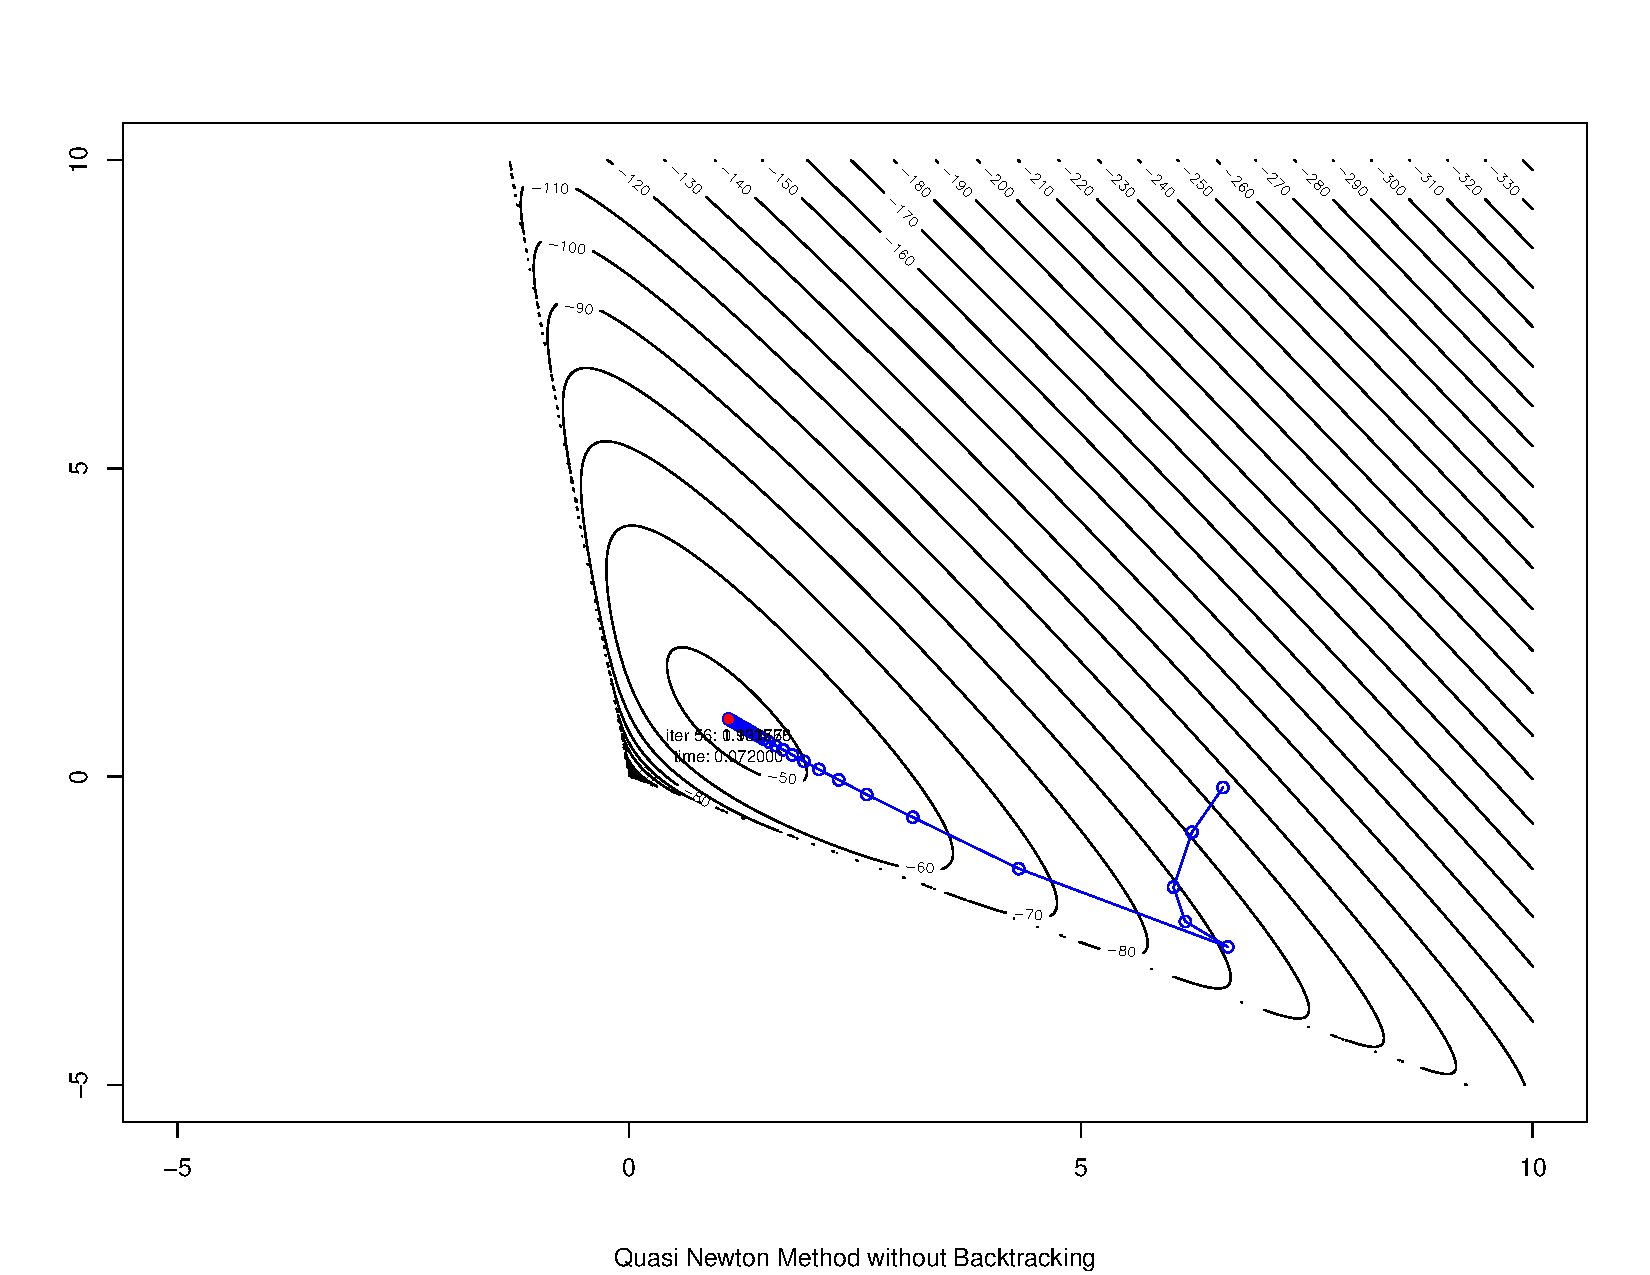
\includegraphics[scale=0.3]{figs/quasi-noback.pdf}
\caption{Quasi-Newton method without backtracking.}
\label{img:quasi-noback}
\end{figure}

\begin{figure}[h!]
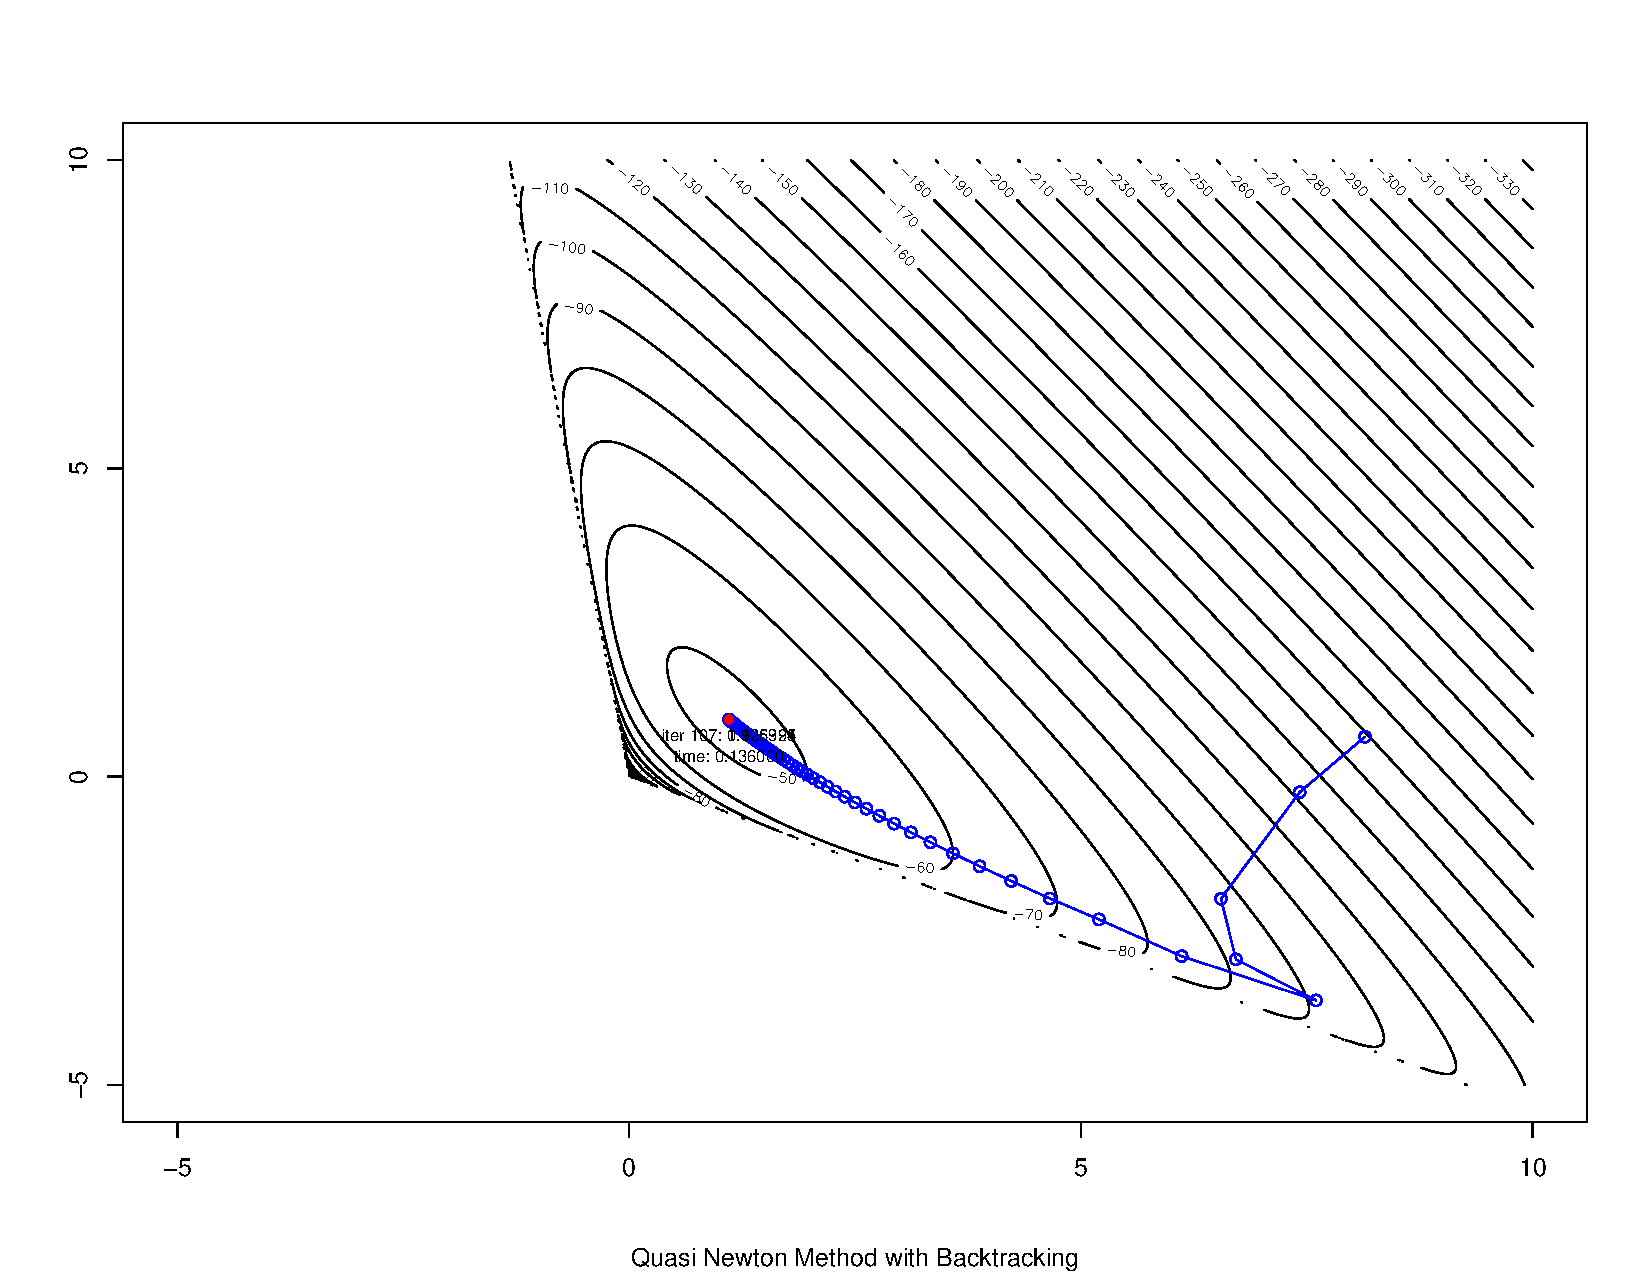
\includegraphics[scale=0.3]{figs/quasi-back.pdf}
\caption{Quasi-Newton method with backtracking.}
\label{img:quasi-back}
\end{figure}

In problem 2.5 \textit{(a)} to \textit{(d)}, we discuss about the performance of \textit{Newton} and \textit{Fisher Scoring} methods for multivariate estimation problem. Specifically, as shown in Fig. \ref{img:newton} and Fig. \ref{img:fisher}, textit{Newton} can only work with initial points in a very limited extent, however, \textit{Fisher Scoring} can work with initial points even at the margin of range in this figure. Similarly, here the red points mean the final solution of local optimal and blue points mean the trace of solutions over iterations. In Fig. \ref{img:std-err-alpha}, we also show the standard error of $\alpha_1$ and $alpha_2$ over iterations in accordance with the requirement of problem 2.5 \textit{(d)}.

In problem 2.5 \textit{(e)} and \textit{(f)}, we further evaluate the influences of backtracking trick when applying on \textit{Quasi-Newton} method and \textit{Steepest Ascent} method. Generally, backtraking trick allows the algorithm make much bolder attempts even the step is downhill. As we can easily tell in Fig. \ref{img:ascent-noback}, Fig. \ref{img:ascent-back}, Fig. \ref{img:quasi-noback} and Fig. \ref{img:quasi-back}, the iteration trace of methods with backtraking look zigzag, sometimes it even make the tentative steps over the local optimal, which usually means fast convergence speed. Comparing to the iteration trace of methods without backtracking, they look smoother than the previous. 

\section{Conclusion}

In sum, we discuss several common optimization methods in this report, and do contrast experiments for each of them. Generally, \textit{Quasi-Newton} is the fastest method for finding local optimal, which is also the most commonly-used method for optimization (like \textit{BFGS}). And backtracking trick can speed some algorithm up under some certain conditions. 

\begin{appendices}
\section{main.R Appendix}
\label{appendix:main}
\begin{lstlisting}[
	basicstyle=\tiny, %or \small or \footnotesize etc.
]
# HW2 - Optimization
# updated at Feb 5, 2018
# by Shixiang (Woody) Zhu

# Configurations
rootPath <- "your/path/to/project/"
dataPath <- paste(rootPath, "datasets/oilspills.dat", sep="/")
source(paste(rootPath, "hw2-optimization/rootfinder.R", sep="/"))
source(paste(rootPath, "hw2-optimization/optimizer.R", sep="/"))
source(paste(rootPath, "hw2-optimization/plotter.R", sep="/"))

# Problem 1:
# ==============================================================================
# The following data are an i.i.d sample from a Cauchy(theta, 1) distribution: 
data <- c(1.77, -0.23, 2.76, 3.80, 3.47, 56.75, -1.34, 4.24, -2.44, 3.29, 3.71, 
          -2.40, 4.53, -0.07, -1.05, -13.87, -2.53, -1.75, 0.27, 43.21)

#    Loglikelihood function of Cauchy distribution (theta, scale=1)
loglikCauchy <- function(location, scale=1., xs=data) {
  sum(dcauchy(xs, location=location, scale=scale, log=TRUE))
}
#    Derivative of loglikelihood function of Cauchy distribution (theta, 1)
derivLoglikCauchy <- function(location, xs=data) { 
  2 * sum((xs - location) / (1 + (xs - location)^2))
}

locations <- seq(-20, 60, 1/50) # Range of medians to plot
scales    <- seq(-5, 5, 1/50)   # Range of (log) scales to plot
u <- as.matrix(expand.grid(locations, exp(scales))) # Points to evaluate
y <- apply(as.matrix(locations), 1, function(v) loglikCauchy(v, 1., data))
z <- matrix(apply(u, 1, function(v) loglikCauchy(v[1], v[2], data)),
            nrow=length(locations))

# ------------------------------------------------------------------------------
# a. Graph the log-likelihood function as location and scale vary
filled.contour(locations, scales, z, color.palette=heat.colors,
               xlab="Location", ylab="Log(scale)",
               main="Cauchy Log Likelihood")

#    Graph the log-likelihood function as only location vary when scale=1.
plot(locations, y, type="l", xlab="locations", ylab="log-likelihood", 
     main="Cauchy Log likelihood (scale=1.)")

#    Find the MLE for theta using the Newton-Raphson method. Try all of the 
#    following starting points: 
startPois <- c(-11, -1, 0, 1.5, 4, 4.7, 7, 8, 38)
#    Discuss your results. Is the mean of the data is a good starting point?

#    Solve Maximum likelihood Estimation by Newton Raphson
newtonMLE <- newtonRaphson(f=derivLoglikCauchy, x0=mean(data))
# #    Plot solutions on their loglikelihood function and its derivative function
# plotSol(locations, derivLoglikCauchy, newtonMLE,
#         xlabel="theta", ylabel="derivative of log likelihood", 
#         subtitle="Derivative of Cauchy Log likelihood (scale=1.)",
#         title="Newton-Raphson")
# plotSol(locations, loglikCauchy, newtonMLE, 
#         xlabel="theta", ylabel="log likelihood", 
#         subtitle="Cauchy Log likelihood (scale=1.)",
#         title="Newton-Raphson",
#         zeroLine=FALSE)

# ------------------------------------------------------------------------------
# b. Apply the bisection method with starting points:
startPois <- c(-1., 1.)
#    Use additional runs to illustrate manners in which the bisection method may 
#    fail to find the global maximum. 

#    Solve Maximum likelihood Estimation by Bisection Method
bisecMLE <- bisection(f=derivLoglikCauchy, a=-1., b=1)

# ------------------------------------------------------------------------------
# c. Apply fixed-point iterations as in (2.29), starting from -1, with scaling 
#    choices of alpha=1, 0.64, and 0.25. Investigate other choices of starting 
#    values and scaling factors.

#    Solve Maximum likelihood Estimation by Fixed Point Method
fixedPoiMLE <- fixedPoint(f=derivLoglikCauchy, x0=-1, alpha=0.64)

# ------------------------------------------------------------------------------
# d. From staring values of (theta^(0), theta^(1)) = (-2, -1), apply the secant 
#    method to estimate theta. What happens when (theta^(0), theta^(1)) = (-3, 3), 
#    and for other starting choices?

#    Solve Maximum likelihood Estimation by Fixed Point Method
secantMLE <- secant(f=derivLoglikCauchy, x0=-3, x1=3)

#    Plot solutions on their loglikelihood function and its derivative function
plotMLE(f=loglikCauchy, 
        newtonMLE, bisecMLE, fixedPoiMLE, secantMLE, 
        xlabel="theta", ylabel="log likelihood", 
        subtitle="Cauchy Log likelihood (scale=1.)",
        zeroLine=FALSE)
plotMLE(f=derivLoglikCauchy, 
        newtonMLE, bisecMLE, fixedPoiMLE, secantMLE, 
        xlabel="theta", ylabel="derivative of log likelihood", 
        subtitle="Derivative of Cauchy Log likelihood (scale=1.)",
        zeroLine=TRUE)

# ------------------------------------------------------------------------------
# e. Use this example to compare the speed and stability of the Newton-Raphson 
#    method, bisection, fixed-point iteration, and the secant method. Do your 
#    conclusions change when you apply the methods to a random sample of size 20 
#    from a N(theta, 1) distribution?

#    Sample data from a N(theta, 1) (theta = 0)
data <- rnorm(20, mean=0., sd=1.)
#    Loglikelihood function of Cauchy distribution (theta, scale=1)
loglikNorm <- function(theta, std=1., xs=data) {
  sum(dnorm(xs, mean=theta, sd=std, log=TRUE))
}
#    Derivative of loglikelihood function of Cauchy distribution (theta, 1)
derivLoglikNorm <- function(theta, xs=data) {
  require(numDeriv)
  genD(func=loglikNorm, x=theta)$D[1]
}

newtonMLE   <- newtonRaphson(f=derivLoglikNorm, x0=mean(data))
bisecMLE    <- bisection(f=derivLoglikNorm, a=-1., b=0)
fixedPoiMLE <- fixedPoint(f=derivLoglikNorm, x0=1, alpha=0.01)
secantMLE   <- secant(f=derivLoglikNorm, x0=-3, x1=3)

plotMLE(f=loglikNorm, 
        newtonMLE, bisecMLE, fixedPoiMLE, secantMLE, 
        zeroLine=FALSE)
plotMLE(f=derivLoglikNorm, 
        newtonMLE, bisecMLE, fixedPoiMLE, secantMLE,
        ylabel="derivative of log likelihood", 
        subtitle="Derivative of Normal Log likelihood (std=1.)",
        zeroLine=TRUE)

# Problem 2:
# ==============================================================================
# There were 46 crude oil spills of at least 1,000 barrels from tankers in U.S. waters 
# during 1974-1999. The website for this book contains the following data: the number
# of spills in the i-th year, N_i; the estimated amount of oil shipped through US waters
# as part of US import/export operations in the i-th year, adjusted for spillage in 
# international or foreign waters, b_i1; and the amount of oil shipped through U.S. 
# waters during domestic shipments in the i-th year, b_i2. The data are adapted from [11].
# Oil shipment amounts are measured in billions of barrels (Bbbl).
# 
# The volume of oil shipped is measure of exposure to spill risk. Suppose we use the 
# Possion process assumption given by N_i | b_i1, b_i2 ~ Possion(lambda_i) where 
# lambda_i = alpha_1 * b_i1 + alpha_2 * b_i2. The parameters of this model are alpha_1 and
# alpha_2, which represent the rate of spill occurence per Bbbl oil shipped during import/
# expert and domestic shipments, respectively. 
spillsData <- read.table(dataPath, header=TRUE)

# (Maximize) Objective function
loglikPoisson <- function(alpha, data=spillsData) {
  sum(dpois(data$spills, alpha[1]*data$importexport + alpha[2]*data$domestic, log=TRUE))
}

# ------------------------------------------------------------------------------
# a. Derive the Newton-Raphson update for finding the MLEs of alpha_1 and alpha_2.
# b. Derive the Fisher scoring update for finding the MLEs of alpha_1 and alpha_2.
# c. Implement the Newton-Raphson and Fisher scoring methods for this problem, 
#    provide the MLEs, and compare the implementation case and performance of 
#    the two methods.
resNewtonMLE <- newtonRaphsonMLE(loglikFunc=loglikPoisson, 
                                 theta0=c(3, -1))
resFisherMLE <- fisherScoringMLE(loglikFunc=loglikPoisson, 
                                 data=spillsData, theta0=c(10, -1))

plot2DMLE(loglikPoisson, resNewtonMLE, "Newton Method")
plot2DMLE(loglikPoisson, resFisherMLE, "Fisher Scoring")

# ------------------------------------------------------------------------------
# d. Estimate standard errors for the MLEs of alpha_1 and alpha_2.
par(mfrow=c(1, 2))
errorAlpha1 <- sqrt((as.vector(resNewtonMLE$iterations[,1]) - 
                               resNewtonMLE$rootApproximation[1])^2)
errorAlpha2 <- sqrt((as.vector(resNewtonMLE$iterations[,2]) - 
                               resNewtonMLE$rootApproximation[2])^2)
plot(errorAlpha1, type="l", xlab="Iteration", ylab="Standard Error for Alpha 1")
plot(errorAlpha2, type="l", xlab="Iteration", ylab="Standard Error for Alpha 2")

# ------------------------------------------------------------------------------
# e. Apply the method of steepest ascent. Use step-halving backtracking as
#    necessary.
resAscentBackMLE <- steepestAscentMLE(loglikFunc=loglikPoisson, theta0=c(3, -1), 
                                      alpha0=0.5)
resAscentMLE     <- steepestAscentMLE(loglikFunc=loglikPoisson, theta0=c(3, -1), 
                                      alpha0=0.05, backtracking=FALSE)
plot2DMLE(loglikPoisson, resAscentBackMLE, "Ascent Method with Backtracking")
plot2DMLE(loglikPoisson, resAscentMLE, "Ascent Method without Backtracking")

# ------------------------------------------------------------------------------
# f. Apply quasi-Newton optimaztion with the Hessian approximation update given 
#    in (2.49). Compare performance with and without step halving.
resQuasiBackMLE <- quasiNewtonMLE(loglikFunc=loglikPoisson, theta0=c(5, -1), 
                                  alpha0=0.2)
resQuasiMLE     <- quasiNewtonMLE(loglikFunc=loglikPoisson, theta0=c(5, -1), 
                                  alpha0=0.1, backtracking=FALSE)
plot2DMLE(loglikPoisson, resQuasiBackMLE, "Quasi Newton Method with Backtracking")
plot2DMLE(loglikPoisson, resQuasiMLE, "Quasi Newton Method without Backtracking")

# ------------------------------------------------------------------------------
# g. Construct a graph resembling Figure 2.8 that compares the paths taken 
#    by methods used in (a)-(f). Choose the plotting region and starting point 
#    to best illustrate the features of the algorithms' performance.
\end{lstlisting}

\section{rootfinder.R Appendix}
\label{appendix:findroot}
\begin{lstlisting}[
	basicstyle=\tiny, %or \small or \footnotesize etc.
]
# Newton Raphson Method
newtonRaphson <- function(f, x0, tol=1e-3, n=1000) {
  # Start the clock!
  ptm <- proc.time()
  
  require(numDeriv) # Package for computing f'(x)
  k <- n # Initialize for iteration results
  
  # Check the upper and lower bounds to see if approximations result in 0
  if (f(x0) == 0.) {
    res <- list("rootApproximation" = x0, "iterations" = c(x0))
  }
  
  for (i in 1:n) {
    dx   <- genD(func=f, x=x0)$D[1] # First-order derivative f'(x0)
    x1   <- x0 - (f(x0) / dx)       # Calculate next value x1
    k[i] <- x1 # Store x1
    # Once the difference between x0 and x1 becomes sufficiently small, 
    # output the results.
    if (abs(x1 - x0) < tol) {
      # Stop the clock
      dt <- proc.time() - ptm
      rootApprox <- tail(k, n=1)
      res <- list("rootApproximation" = rootApprox, 
                  "iterations" = k, 
                  "time" = dt,
                  "methodName" = "Newton Raphson")
      return(res)
    }
    # If Newton-Raphson has not yet reached convergence set x1 as x0 and continue
    x0 <- x1
  }
  stop("Exceeded allowed number of iterations")
}

# Bisection Method
bisection <- function(f, a, b, tol=1e-3, n=1000) {
  # Start the clock!
  ptm <- proc.time()
  
  k <- n # Initialize for iteration results
  
  # If the signs of the function at the evaluated points, a and b, 
  # stop the function and return message.
  if (!(f(a) < 0) && (f(b) > 0)) {
    stop('signs of f(a) and f(b) differ')
  } 
  else if (!(f(a) > 0) && (f(b) < 0)) {
    stop('signs of f(a) and f(b) differ')
  }
  
  for (i in 1:n) {
    c <- (a + b) / 2 # Calculate midpoint
    k[i] <- c
    # If the function equals 0 at the midpoint or the midpoint is 
    # below the desired tolerance, stop the 
    # function and return the root.
    if ((f(c) == 0) || ((b - a) / 2) < tol) {
      # Stop the clock
      dt <- proc.time() - ptm
      rootApprox <- tail(k, n=1)
      res <- list("rootApproximation" = rootApprox, 
                  "iterations" = k, 
                  "time" = dt,
                  "methodName" = "Bisection")
      return(res)
    }
    
    # If another iteration is required, 
    # check the signs of the function at the points c and a and reassign
    # a or b accordingly as the midpoint to be used in the next iteration.
    ifelse(sign(f(c)) == sign(f(a)), 
           a <- c,
           b <- c)
  }
  # If the max number of iterations is reached and no root has been found, 
  # return message and end function.
  stop("Exceeded allowed number of iterations")
}

# Fixed Point Method
fixedPoint <- function(f, x0, alpha=1, tol=1e-02, n=1000){
  # fixed-point algorithm to find x such that x + f(x) == x
  # assume that fun is a function of a single variable
  # x0 is the initial guess at the fixed point
  
  # Start the clock!
  ptm <- proc.time()
  
  k <- n # Initialize for iteration results
  
  if (f(x0) == 0){
    res <- list("rootApproximation" = x0, "iterations" = c(x0))
  }
  for (i in 1:n) {
    x1   <- x0 + alpha * f(x0) 
    k[i] <- x1
    if ( abs((x1 - x0)) < tol ) {
      # Stop the clock
      dt <- proc.time() - ptm
      rootApprox <- tail(k, n=1)
      res <- list("rootApproximation" = rootApprox, 
                  "iterations" = k, 
                  "time" = dt,
                  "methodName" = "Fixed Point")
      return(res)
    }
    x0 <- x1
  } 
  stop("Exceeded allowed number of iterations")
}

secant <- function(f, x0, x1, tol=1e-03, n=1000){
  # Start the clock!
  ptm <- proc.time()
  
  k <- n # Initialize for iteration results
  
  for ( i in 1:n ) {
    x2   <- x1 - f(x1) * (x1 - x0) / (f(x1) - f(x0))
    k[i] <- x2
    if (abs(f(x2)) < tol) {
      # Stop the clock
      dt <- proc.time() - ptm
      rootApprox <- tail(k, n=1)
      res <- list("rootApproximation" = rootApprox, 
                  "iterations" = k,
                  "time" = dt,
                  "methodName" = "Secant")
      return(res)
    }
    x0 <- x1
    x1 <- x2
  }
  stop("Exceeded allowed number of iteractions")
}
\end{lstlisting}

\section{optimizer.R Appendix}
\label{appendix:optimizer}
\begin{lstlisting}[
	basicstyle=\tiny, %or \small or \footnotesize etc.
]
library(MASS)

newtonRaphsonMLE <- function(loglikFunc, theta0, tol=1e-9, n=1000) {
  # Start the clock!
  ptm <- proc.time()
  
  require(numDeriv) # Package for computing f'(x) and f''(x)
  k <- matrix(0, ncol=length(theta0)) # Initialize for iteration results
  
  for (i in 1:n) {
    deriv  <- genD(func=loglikFunc, x=theta0)$D[1:length(theta0)] 
    hess   <- hessian(func=loglikFunc, x=theta0)                  
    theta1 <- theta0 - deriv %*% solve(hess)  # Calculate next value theta1 
    k      <- rbind(k, theta1)                # Store theta1

    # Once the difference between theta0 and theta1 becomes sufficiently small, 
    # output the results.
    if (sum(abs(theta1 - theta0)) < tol) {
      # Stop the clock
      dt <- proc.time() - ptm
      rootApprox <- tail(k, n=1)
      res <- list("rootApproximation" = rootApprox, 
                  "iterations" = tail(k, n=i), 
                  "time" = dt,
                  "methodName" = "Newton Raphson")
      return(res)
    }
    # If Newton-Raphson has not yet reached convergence set theta1 as theta0 
    # and continue
    theta0 <- theta1
  }
  stop("Exceeded allowed number of iterations")
}

fisherScoringMLE <- function(loglikFunc, data, theta0, 
                             tol=1e-3, n=1000) {
  # Start the clock!
  ptm <- proc.time()
  
  require(numDeriv) # Package for computing f'(x) and f''(x)
  k <- matrix(0, ncol=length(theta0)) # Initialize for iteration results
  
  for (i in 1:n) {
    # Score of loglikelihood 
    score      <- genD(func=loglikFunc, x=theta0)$D[1:length(theta0)] 
    # Fisher Information of loglikelihood
    fisherInfo <- matrix(0, ncol=length(theta0), nrow=length(theta0))
    for (j in 1:nrow(data)) {
      estFunc <- function(theta, d=data[j,]) { loglikFunc(theta, d) }
      estVec  <- genD(func=estFunc, x=theta0)$D[1:length(theta0)]
      fisherInfo <- fisherInfo + estVec%*%t(estVec)
    }
    # Update theta by fisher scoring
    theta1 <- theta0 + MASS::ginv(fisherInfo) %*% score
    k      <- rbind(k, t(theta1)) # Store theta1
    if (sum(abs(theta1 - theta0)) < tol) {
      # Stop the clock
      dt <- proc.time() - ptm
      rootApprox <- tail(k, n=1)
      res <- list("rootApproximation" = rootApprox, 
                  "iterations" = tail(k, n=i), 
                  "time" = dt,
                  "methodName" = "Fisher Scoring")
      return(res)
    }
    theta0 <- theta1
  }
  stop("Exceeded allowed number of iterations")
}

steepestAscentMLE <- function(loglikFunc, theta0, alpha0=1., 
                              tol=1e-3, n=1000, backtracking=TRUE) {
  # Start the clock!
  ptm <- proc.time()
  
  require(numDeriv) # Package for computing f'(x) and f''(x)
  k <- matrix(0, ncol=length(theta0)) # Initialize for iteration results
  
  alpha <- alpha0
  for (i in 1:n) {
    deriv  <- genD(func=loglikFunc, x=theta0)$D[1:length(theta0)] 
    # Steepest ascent
    h      <- -1 * alpha * solve(-1 * diag(length(theta0))) %*% deriv
    # Update theta
    theta1 <- theta0 + alpha * deriv
    k      <- rbind(k, t(theta1)) # Store theta1
    # Backtracking by updating alpha
    if (backtracking && (loglikFunc(theta0) - loglikFunc(theta1) > 0.)) {
      alpha <- alpha * 0.5
    }
    if (sum(abs(theta1 - theta0)) < tol) {
      # Stop the clock
      dt <- proc.time() - ptm
      rootApprox <- tail(k, n=1)
      res <- list("rootApproximation" = rootApprox, 
                  "iterations" = tail(k, n=i), 
                  "time" = dt,
                  "methodName" = "Fisher Scoring")
      return(res)
    }
    theta0 <- theta1
  }
  stop("Exceeded allowed number of iterations")
}

quasiNewtonMLE <- function(loglikFunc, theta0, alpha0=1, 
                           tol=1e-3, n=1000, backtracking=TRUE) {
  # Start the clock!
  ptm <- proc.time()
  
  k <- matrix(0, ncol=length(theta0)) # Initialize for iteration results
  # An initial matrix M0 is chosen (usually M0 = I)
  M <- diag(length(theta0))
  # An initial alpha alpha0 is chosen
  alpha <- alpha0
  for (i in 1:n) {
    # Update theta
    deriv0 <- genD(func=loglikFunc, x=theta0)$D[1:length(theta0)]
    theta1 <- theta0 - alpha * solve(M) %*% deriv0
    deriv1 <- genD(func=loglikFunc, x=theta1)$D[1:length(theta1)]
    # Update Matrix M
    z <- as.vector(theta1 - theta0)
    y <- deriv1 - deriv0
    v <- y - M %*% z
    c <- solve(t(v) %*% z)
    M <- M + c[1] * (v %*% t(v))
    # Backtracking by updating alpha
    if (backtracking && (loglikFunc(theta0) - loglikFunc(theta1) > 0.)) {
      alpha <- alpha * 0.5
    }
    # Update theta
    k <- rbind(k, t(theta1)) # Store theta1
    if (sum(abs(theta1 - theta0)) < tol) {
      # Stop the clock
      dt <- proc.time() - ptm
      rootApprox <- tail(k, n=1)
      res <- list("rootApproximation" = rootApprox, 
                  "iterations" = tail(k, n=i),
                  "time" = dt,
                  "methodName" = "Fisher Scoring")
      return(res)
    }
    theta0 <- theta1
  }
  stop("Exceeded allowed number of iterations")
}
\end{lstlisting}

\section{plotter.R Appendix}
\label{appendix:plotter}
\begin{lstlisting}[
	basicstyle=\tiny, %or \small or \footnotesize etc.
]
plotSol <- function (x, yLoglikFunc, resMLE, 
                     xlabel, ylabel, subtitle, title, 
                     zeroLine=TRUE) {
  # Variables Configurations
  y           <- apply(as.matrix(x), 1, function(v) yLoglikFunc(v))
  xIters      <- resMLE$iterations 
  yIters      <- apply(as.matrix(xIters), 1, function(v) yLoglikFunc(v))
  labelIters  <- cbind(1:length(xIters), xIters)
  namebank    <- apply(as.matrix(labelIters), 1, 
                       function(v) sprintf("iter %d: %f", v[1], v[2]))
  # Plot derivative of loglikelihood function
  plot(x, y, type="l", xlab=xlabel, ylab=ylabel, sub=subtitle, main=title)
  if (zeroLine) {
    abline(h = 0, lty = 2)
  }
  points(xIters, yIters, pch=16, col="blue")
  points(resMLE$rootApproximation, # Root x
         yLoglikFunc(resMLE$rootApproximation), 
         pch=20, col="red")
  text(resMLE$rootApproximation,   # Root x
       yLoglikFunc(resMLE$rootApproximation),
       labels=sprintf("iter %d: %f\ntime: %f", length(xIters), resMLE$rootApproximation, resMLE$time[1]), 
       cex= 0.7, pos=1)
}

plotMLE <- function (f, newtonMLE, bisecMLE, fixedPoiMLE, secantMLE, 
                     step=1/50, xrange=c(-30, 30),
                     xlabel="theta", ylabel="log likelihood", 
                     subtitle="Normal Log likelihood (std=1.)",
                     zeroLine=TRUE) {
  par(mfrow=c(2,2))
  xs <- seq(xrange[1], xrange[2], step) # Range of means to plot
  plotSol(xs, f, newtonMLE, 
          xlabel=xlabel, ylabel=ylabel, subtitle=subtitle, 
          title=newtonMLE$methodName, zeroLine=zeroLine)
  plotSol(xs, f, bisecMLE, 
          xlabel=xlabel, ylabel=ylabel, subtitle=subtitle, 
          title=bisecMLE$methodName, zeroLine=zeroLine)
  plotSol(xs, f, fixedPoiMLE, 
          xlabel=xlabel, ylabel=ylabel, subtitle=subtitle, 
          title=fixedPoiMLE$methodName, zeroLine=zeroLine)
  plotSol(xs, f, secantMLE, 
          xlabel=xlabel, ylabel=ylabel, subtitle=subtitle, 
          title=secantMLE$methodName, zeroLine=zeroLine)
}

plot2DMLE <- function(f, resMLE, subtitle, 
                      xlim=c(-5, 10), ylim=c(-5, 10), step=1/50) {
  x <- seq(xlim[1], xlim[2], step)
  y <- seq(ylim[1], ylim[2], step)
  u <- as.matrix(expand.grid(x, y)) # Points to evaluate
  z <- matrix(apply(u, 1, function(v) f(v)), nrow=length(x))
  contour(x, y, z, nlevels=30, sub=subtitle)
  # points(resMLE$iterations[,1], resMLE$iterations[,2], pch=16, col="blue")
  lines(resMLE$iterations[,1], resMLE$iterations[,2], 
        type="o", col="blue") 
  points(resMLE$rootApproximation[1], resMLE$rootApproximation[2],
         pch=20, col="red")
  text(resMLE$rootApproximation[1], resMLE$rootApproximation[2],
       labels=sprintf("iter %d: %f\ntime: %f", 
                      length(resMLE$iterations[,1]), 
                      resMLE$rootApproximation, 
                      resMLE$time[1]), 
       cex= 0.7, pos=1)
}
\end{lstlisting}

\end{appendices}

